\documentclass[12pt]{article}
\usepackage[utf8]{inputenc}
\usepackage[spanish]{babel}
\usepackage{graphicx}
\usepackage{float} 
\usepackage{url}
\usepackage{listingsutf8}
\usepackage{color}
%\usepackage{listingsutf8}
%\usepackage{amsmath,amssymb}
\usepackage[nottoc,notlot,notlof]{tocbibind} % Hace que se agregen las referencias al indice

\definecolor{codegreen}{rgb}{0,0.6,0}
\definecolor{codegray}{rgb}{0.5,0.5,0.5}
\definecolor{codepurple}{rgb}{0.58,0,0.82}
\definecolor{backcolour}{rgb}{0.95,0.95,0.92}

\lstdefinestyle{mystyle}{
	backgroundcolor=\color{backcolour},   
	commentstyle=\color{codegreen},
	keywordstyle=\color{magenta},
	numberstyle=\tiny\color{codegray},
	stringstyle=\color{codepurple},
	basicstyle=\footnotesize,
	breakatwhitespace=false,         
	breaklines=true,                 
	captionpos=b,                    
	keepspaces=true,                 
	numbers=left,                    
	numbersep=5pt,                  
	showspaces=false,                
	showstringspaces=false,
	showtabs=false,                  
	tabsize=2
}

\lstset{
	style=mystyle,
	inputencoding=utf8/latin1
}

% Title Page
\title{Máquina de Turing que duplica cadena de unos}
\author{Alumno: Monroy Martos Elioth \\ Profesor: Genaro Juárez Martínez \\ Materia: Computing Selected Topics \\ Grupo: 3CM8}


\begin{document}
\maketitle
\newpage
\tableofcontents
\newpage
\section{Introducción}
El formato de archivos de audio digital wav (o wave), es un formato sin compresión de datos que fue desarrollado por Microsoft e IBM, es utilizado para almacenar sonidos en una computadora. Admite archivos mono y estéreos (un canal o dos respectivamente) a diversas resoluciones y velocidades de muestreo.\\ Debido a que no presenta pérdida de calidad, es comúnmente usado profesionalmente para guardar audio en CDs o DVDs. Pero tiene como desventaja, que los archivos creados bajo este formato son bastante grandes en comparación con otros formatos comprimidos como mp3 u ogg.\\ El formato de archivos wav es una variante del formato RIFF (formato de archivo para el intercambio de recursos). Un archivo en formato RIFF, empieza con una cabecera de archivo (file header) seguida de una secuencia de fragmentos de datos (data chunks). Un archivo wav comúnmente, es solo un archivo RIFF pero con una sola ''wave'' chunk, la cual esta formada por dos sub-chunks (fmt sub-chunk y data sub-chunk). A esta forma se le conoce como la forma ''canónica'' de un archivo en formato wav.\\
A continuación se presenta una lista con todos los campos que almacenan la información dentro del archivo wav:
\begin{itemize}
	\item ChunkID (4 bytes): Contiene las letras ''RIFF'' en ascii.
	\item ChunkSize (4 bytes): Es el tamaño del archivo entero menos los 8 bytes de los campos anteriores que no son contados.
	\item Format (4 bytes): Contiene las letras ''WAVE''.
	\item Subchunk1ID (4 bytes): Contiene las letras ''fmt''.
	\item Subchunk1Size (4 bytes): Contiene el tamaño del resto del subchunk que queda a partir de este número.
	\item AudioFormat (2 bytes): Regularmente almacena el número 1, si se guarda algún otro número este indica algún tipo de compresión.
	\item NumChannels (2 bytes): 1 para mono, 2 para stereo.
	\item SampleRate (4 bytes): La frecuencia de muestreo que se uso para muestrear el archivo (8000, 44100, etc).
	\item ByteRate (4 bytes): Es igual a: SampleRate*NumChannels*BitsPerSample/8.
	\item BlockAlign (2 bytes): Guarda el número de bytes por cada muestra (considerando todos los canales). Se obtiene mediante: NumChannels*BitsPerSample/8.
	\item BitsPerSampl (2 bytes): La cantidad de bits que se almacenan por muestra (8 bits, 16 bits, etc).
	\item SubChunk2ID (4 bytes): Contiene las letras ''data''.
	\item SubChunk2Size (4 bytes): Es el número de bytes de los datos, también puede considerarse como el resto del subchunk apartir de este dato.
	\item Data (tamaño del SubChunk2Size): Son los datos del sonido almacenado. 
\end{itemize}
Los campos ChunkID, ChunkSize y Format componen la cabecera del archivo. Los campos Subchunk1ID, Subchunk1Size, AudioFormat, NumChannels, SampleRate, ByteRate, BlockAlign y BitsPerSample componen el primer sub-chunk llamado fmt. Los campos Subchunk2ID, Subchunk2Size y data componen el segundo sub-chunk llamado data.\\ La figura 1 muestra de forma gráfica las cabeceras y campos antes descritos:
\begin{figure}[H]
	\centering
	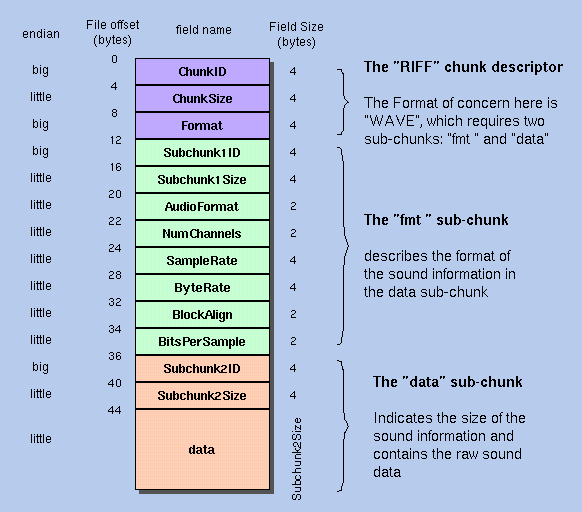
\includegraphics[scale=.7]{img/cabeceras.png}
	\caption{Campos que componen un archivo canónico wav}
	\label{fig:cabeceras}		
\end{figure}

\newpage
\section{Código}
A continuación se presenta el código del programa desarrollado que permite cambiar el volumen a un archivo en formato wav, el programa reduce el volumen del sonido a la mitad (lo cual resulta equivalente a dividir entre dos cada muestra en el archivo).\\
funciones.h:
\begin{lstlisting}[style=CStyle]
#ifndef __FUNCIONES_H__
#define __FUNCIONES_H__
	//Librerías de C
	#include <stdio.h>
	#include <stdlib.h>
	//Métodos
	void leerCabeceras(char**);
	void leerMuestras(short*);
	void dividirMuestras(short*,float);
	void escribirArchivo(short*);
	//Cabeceras
	int chunkid;
	int chunksize;
	int format;
	int subchunk1id;
	int subchunk1size;
	short audioformat;
	short numchannels;
	int samplerate;
	int byterate;
	short blockalign;
	short bitspersample;
	int subchunk2id;
	int subchunk2size;
	//Archivos
	FILE* entrada;
	FILE* salida;
	//Variables para muestras
	short muestra;
	int total_muestras;
	short headers[37];
#endif
\end{lstlisting}
\newpage
half.c:
\begin{lstlisting}[style=CStyle]
#include"funciones.h"
int main(int argc, char *argv[]){
	//Leo las cabeceras
	leerCabeceras(argv);
	//Defino variables
	total_muestras=subchunk2size/blockalign;
	short muestras[total_muestras];
	//Leo las muestras
	leerMuestras(muestras);
	//Divido el volumen a la mitad
	dividirMuestras(muestras,.5);
	//Escribo el archivo
	escribirArchivo(muestras);
}
void leerCabeceras(char ** argv){
	//Abrir archivos
	entrada = fopen(argv[1], "rb");
	salida=fopen(argv[2],"wb");
	if(!entrada) {
		perror("\nFile opening failed");
		exit(0);
	}
	fread(&chunkid,sizeof(int),1,entrada);
	fread(&chunksize,sizeof(int),1,entrada);
	fread(&format,sizeof(int),1,entrada);
	fread(&subchunk1id,sizeof(int),1,entrada);
	fread(&subchunk1size,sizeof(int),1,entrada);
	fread(&audioformat,sizeof(short),1,entrada);
	fread(&numchannels,sizeof(short),1,entrada);
	fread(&samplerate,sizeof(int),1,entrada);
	fread(&byterate,sizeof(int),1,entrada);
	fread(&blockalign,sizeof(short),1,entrada);
	fread(&bitspersample,sizeof(short),1,entrada);
	fread(&subchunk2id,sizeof(int),1,entrada);
	fread(&subchunk2size,sizeof(int),1,entrada);
}
void leerMuestras(short *muestras){
	int i=0;
	while (feof(entrada) == 0)
	{
		if(i<total_muestras){
			fread(&muestra,sizeof(short),1,entrada);
			muestras[i]=muestra;
			i++;
		}else{
			fread(&headers,sizeof(short),37,entrada);
			break;
		}
	}
}
void dividirMuestras(short *muestras, float factor){
	int i;
	for (i = 0; i < total_muestras; i++)
		{
			muestras[i]*=factor;
		}
}
void escribirArchivo(short* muestras){
	//Escribo el archivo
	fwrite(&chunkid,sizeof(int),1,salida);
	fwrite(&chunksize,sizeof(int),1,salida);
	fwrite(&format,sizeof(int),1,salida);
	fwrite(&subchunk1id,sizeof(int),1,salida);
	fwrite(&subchunk1size,sizeof(int),1,salida);
	fwrite(&audioformat,sizeof(short),1,salida);
	fwrite(&numchannels,sizeof(short),1,salida);
	fwrite(&samplerate,sizeof(int),1,salida);
	fwrite(&byterate,sizeof(int),1,salida);
	fwrite(&blockalign,sizeof(short),1,salida);
	fwrite(&bitspersample,sizeof(short),1,salida);
	fwrite(&subchunk2id,sizeof(int),1,salida);
	fwrite(&subchunk2size,sizeof(int),1,salida);
	//Ahora escribo las muestras
	int i=0;
	for(i=0;i<total_muestras;i++){
		fwrite(&muestras[i],sizeof(short),1,salida);
	}
	//Y por último los headers de goldwave
	for(i=0;i<37;i++){
		fwrite(&headers[i],sizeof(short),1,salida);
	}
}
\end{lstlisting}
\newpage
\subsection{Pruebas y resultados}

	\begin{figure}[H]
		\begin{center}
			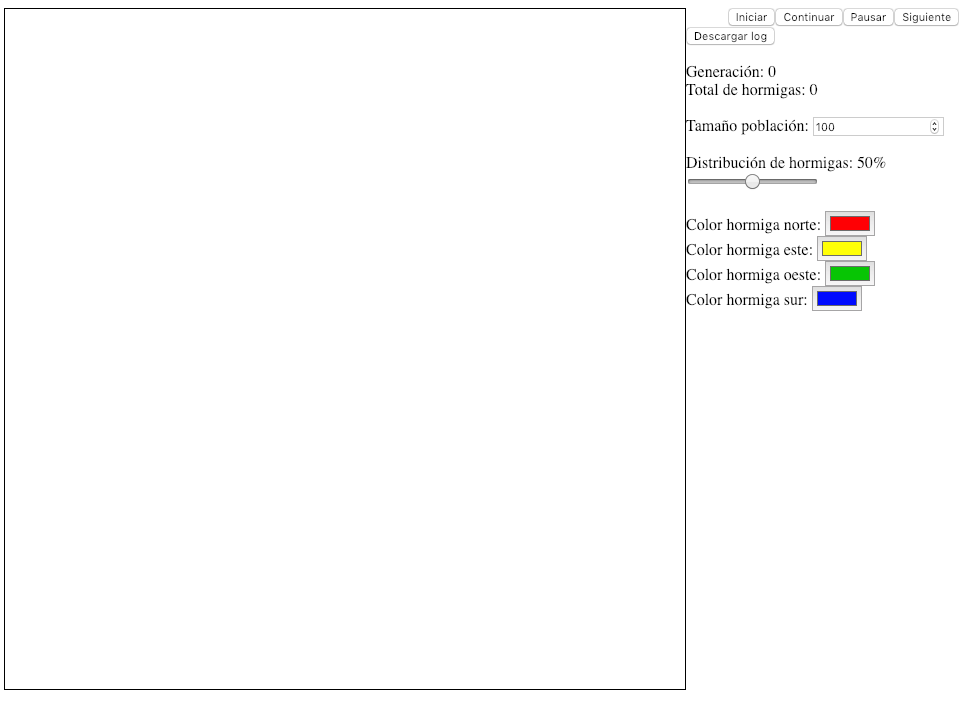
\includegraphics[scale=.3]{GOL/img/interfaz.png}
			\caption{Interfaz gráfica del programa}
			\label{fig:gol1}
		\end{center}
	\end{figure}

	\begin{figure}[H]
		\begin{center}
			
\includegraphics[scale=.5]{GOL/img/1.png}
			\caption{Prueba 1}
			\label{fig:gol2}
		\end{center}
	\end{figure}

	\begin{figure}[H]
		\begin{center}
			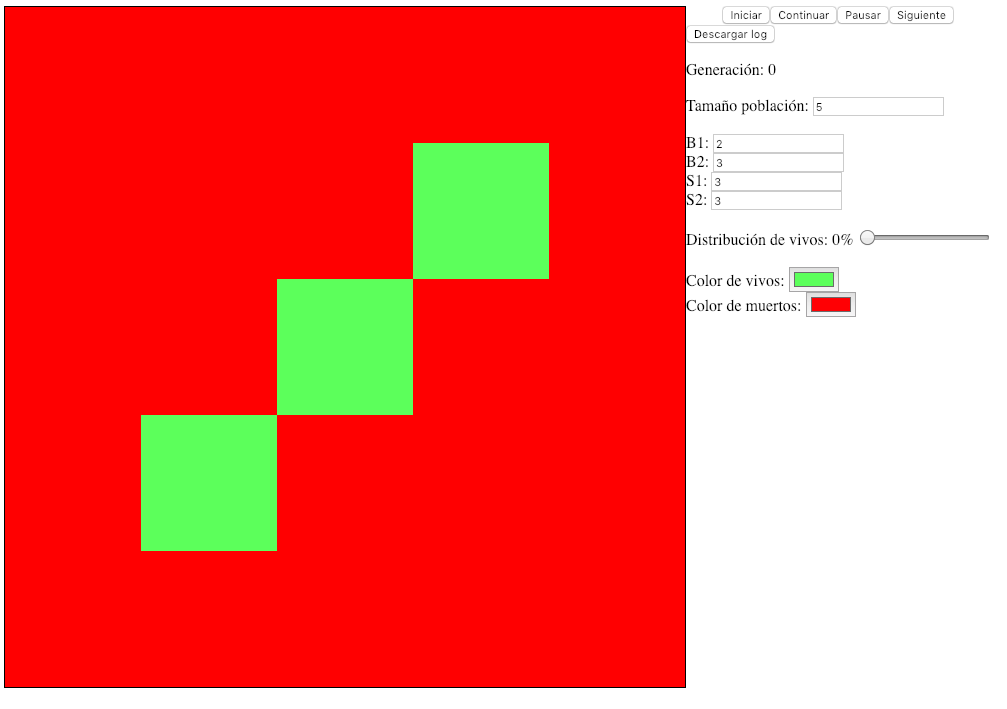
\includegraphics[scale=.3]{GOL/img/test1-1.png}
			\caption{Resultado para la prueba 1 (1)}
			\label{fig:gol3}
		\end{center}
	\end{figure}

	\begin{figure}[H]
		\begin{center}
			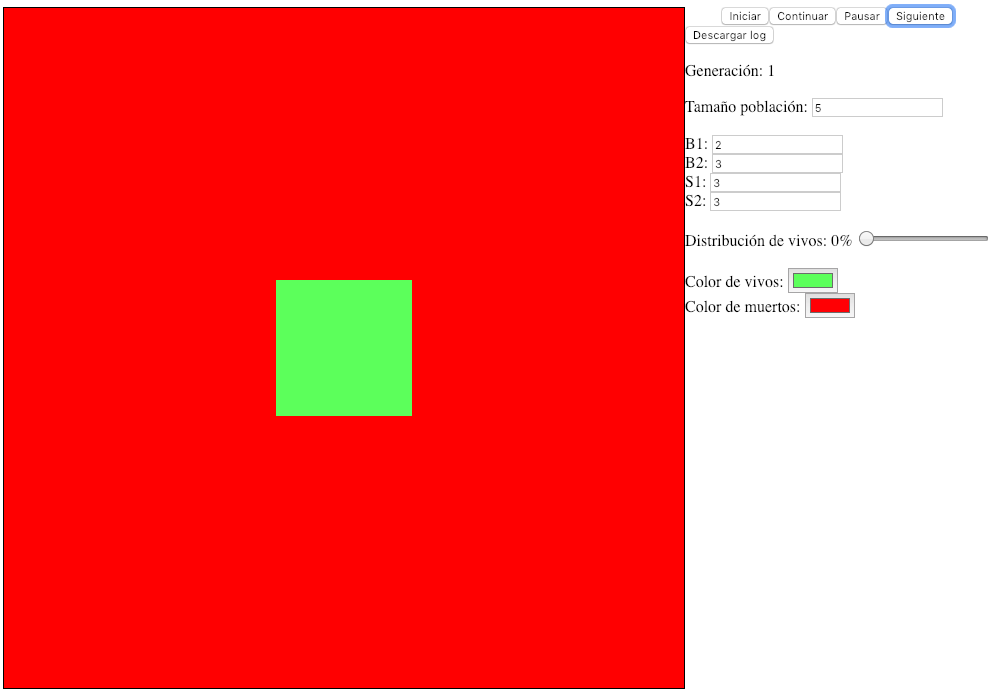
\includegraphics[scale=.3]{GOL/img/test1-2.png}
			\caption{Resultado para la prueba 1 (2)}
			\label{fig:gol4}
		\end{center}
	\end{figure}

	\begin{figure}[H]
		\begin{center}
			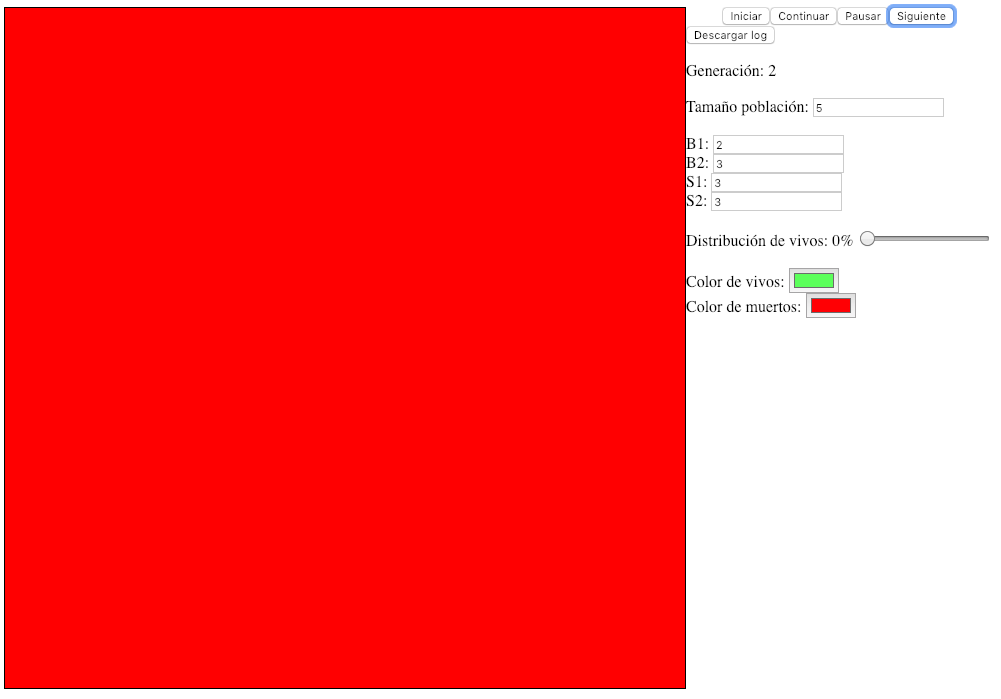
\includegraphics[scale=.3]{GOL/img/test1-3.png}
			\caption{Resultado para la prueba 1 (3)}
			\label{fig:gol5}
		\end{center}
	\end{figure}

	\begin{figure}[H]
		\begin{center}
			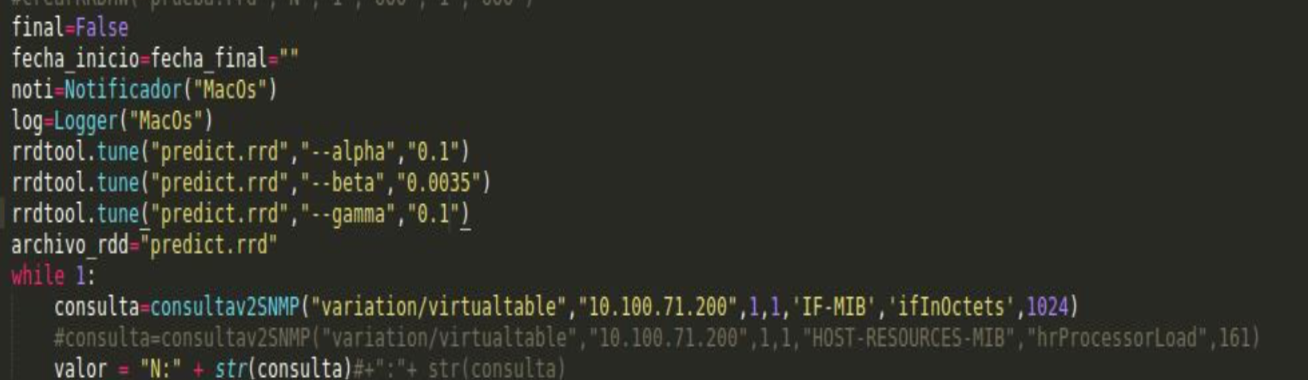
\includegraphics[scale=.5]{GOL/img/2.png}
			\caption{Prueba 2}
			\label{fig:gol4}
		\end{center}
	\end{figure}

	\begin{figure}[H]
		\begin{center}
			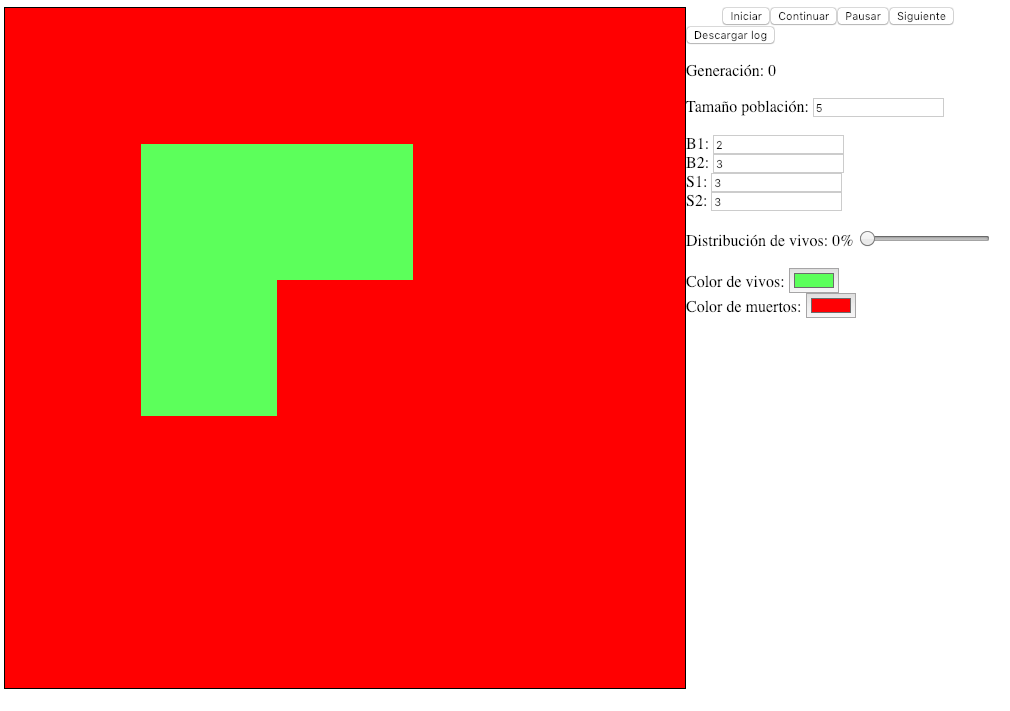
\includegraphics[scale=.3]{GOL/img/test2-1.png}
			\caption{Resultado para la prueba 2 (1)}
			\label{fig:gol5}
		\end{center}
	\end{figure}

	\begin{figure}[H]
		\begin{center}
			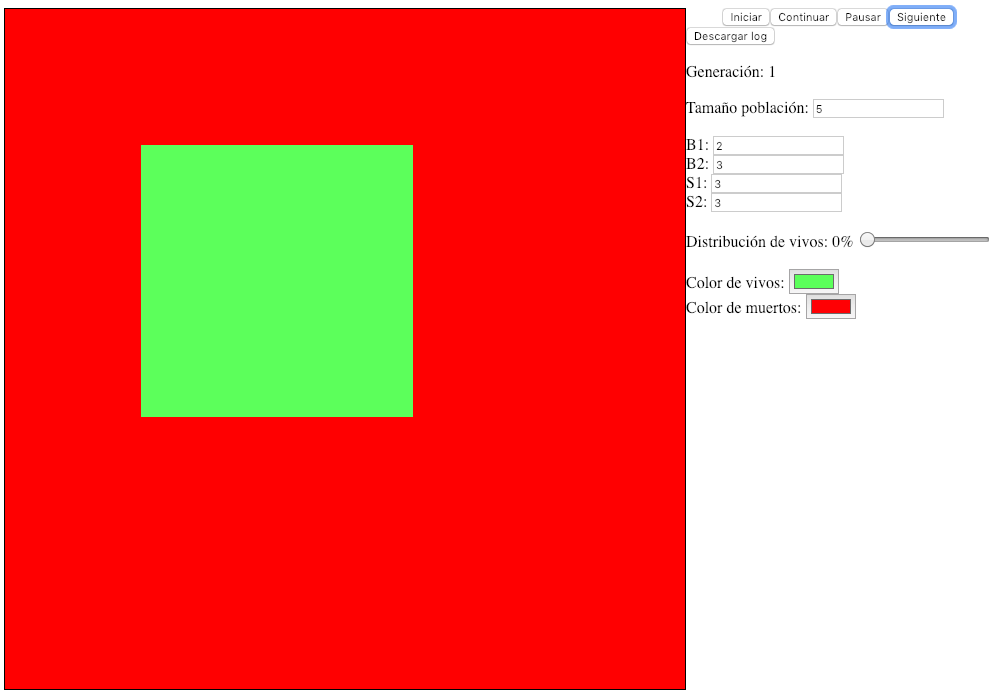
\includegraphics[scale=.3]{GOL/img/test2-2.png}
			\caption{Resultado para la prueba 2 (2)}
			\label{fig:gol4}
		\end{center}
	\end{figure}

	\begin{figure}[H]
		\begin{center}
			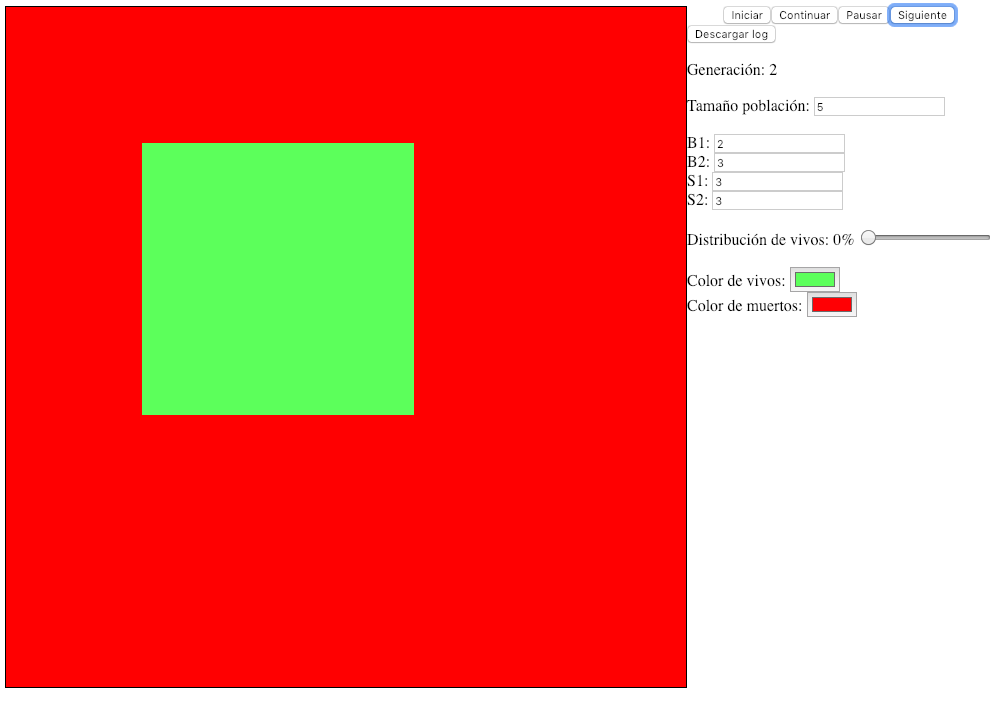
\includegraphics[scale=.3]{GOL/img/test2-3.png}
			\caption{Resultado para la prueba 2 (3)}
			\label{fig:gol5}
		\end{center}
	\end{figure}

	\begin{figure}[H]
		\begin{center}
			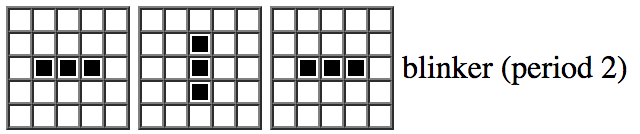
\includegraphics[scale=.5]{GOL/img/3.png}
			\caption{Prueba 3}
			\label{fig:gol4}
		\end{center}
	\end{figure}

	\begin{figure}[H]
		\begin{center}
			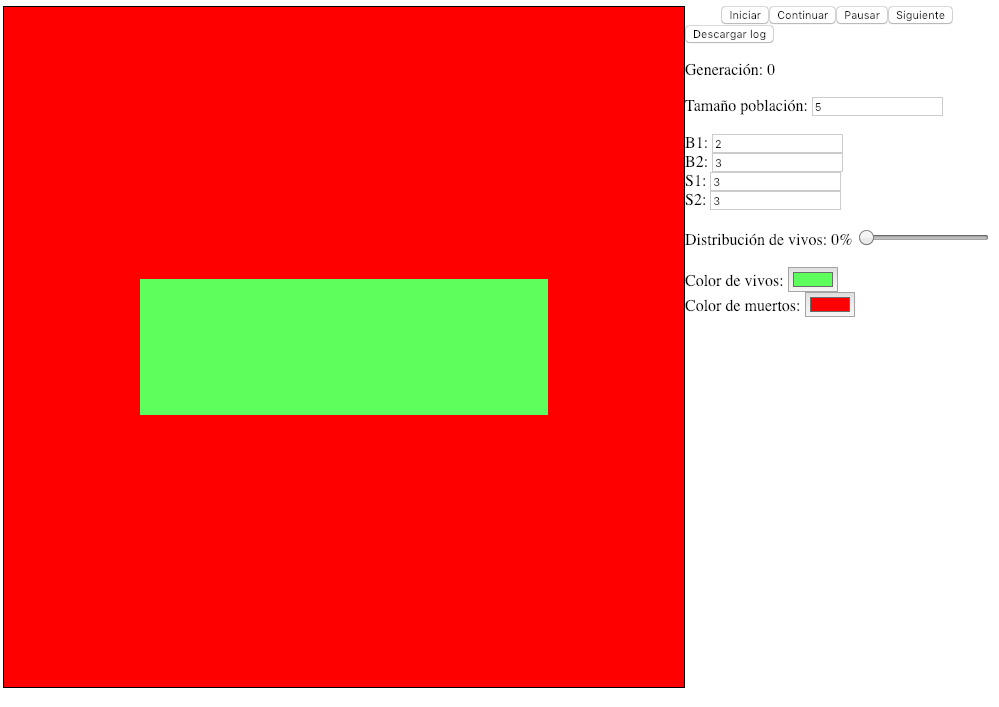
\includegraphics[scale=.3]{GOL/img/test3-1.png}
			\caption{Resultado para la prueba 3 (1)}
			\label{fig:gol5}
		\end{center}
	\end{figure}

	\begin{figure}[H]
		\begin{center}
			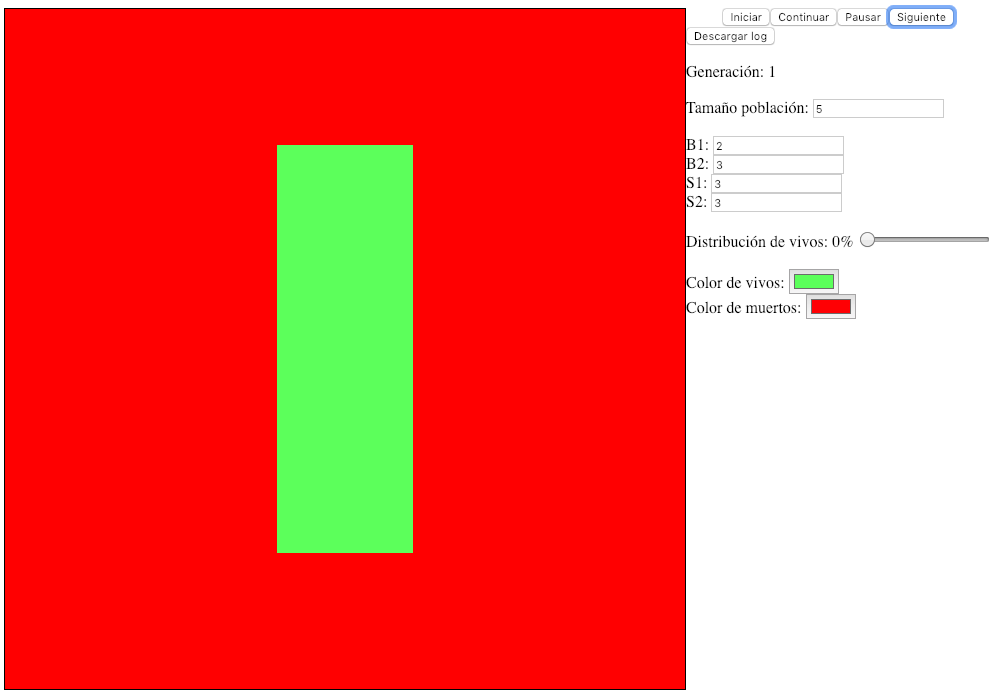
\includegraphics[scale=.3]{GOL/img/test3-2.png}
			\caption{Resultado para la prueba 3 (2)}
			\label{fig:gol4}
		\end{center}
	\end{figure}

	\begin{figure}[H]
		\begin{center}
			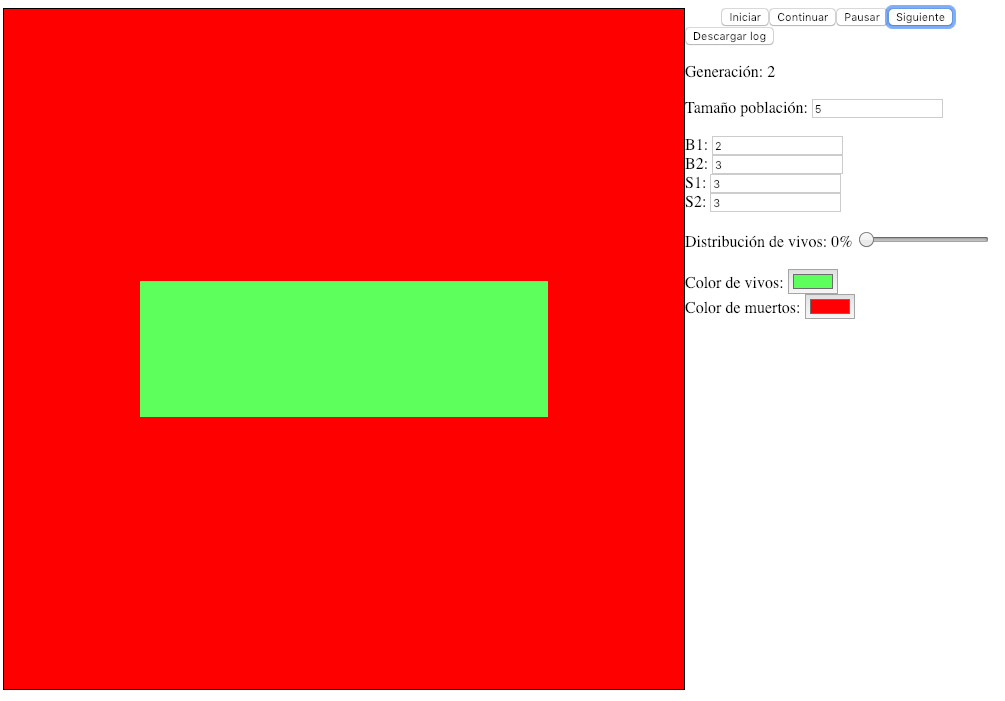
\includegraphics[scale=.3]{GOL/img/test3-3.png}
			\caption{Resultado para la prueba 3 (3)}
			\label{fig:gol5}
		\end{center}
	\end{figure}

	\begin{figure}[H]
		\begin{center}
			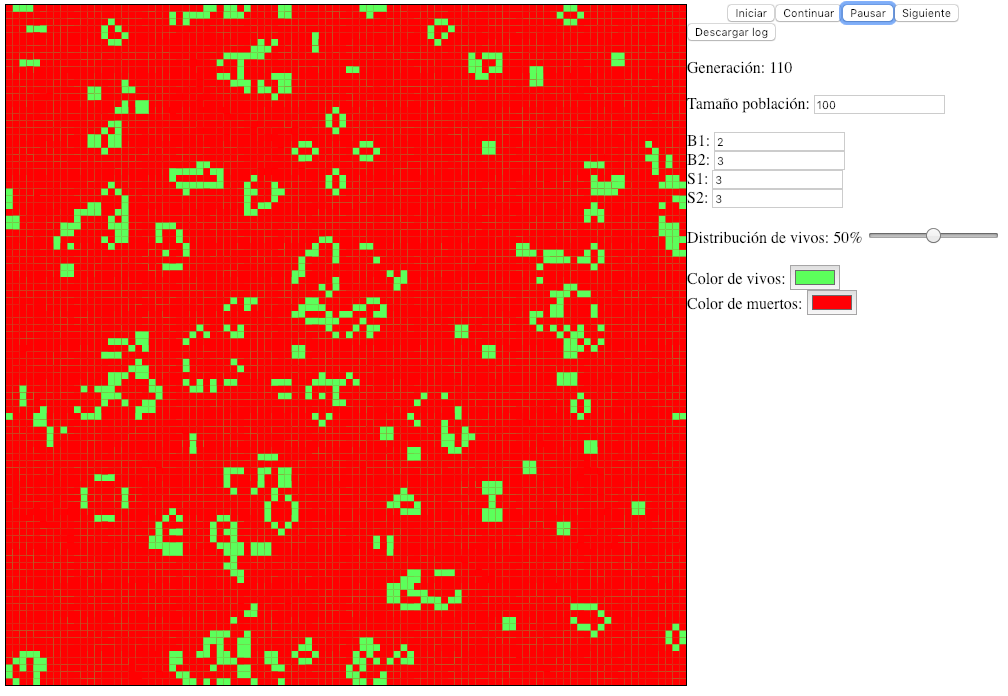
\includegraphics[scale=.3]{GOL/img/life1.png}
			\caption{Juego de la vida después de 100 generaciones}
			\label{fig:gol5}
		\end{center}
	\end{figure}

	\begin{figure}[H]
		\begin{center}
			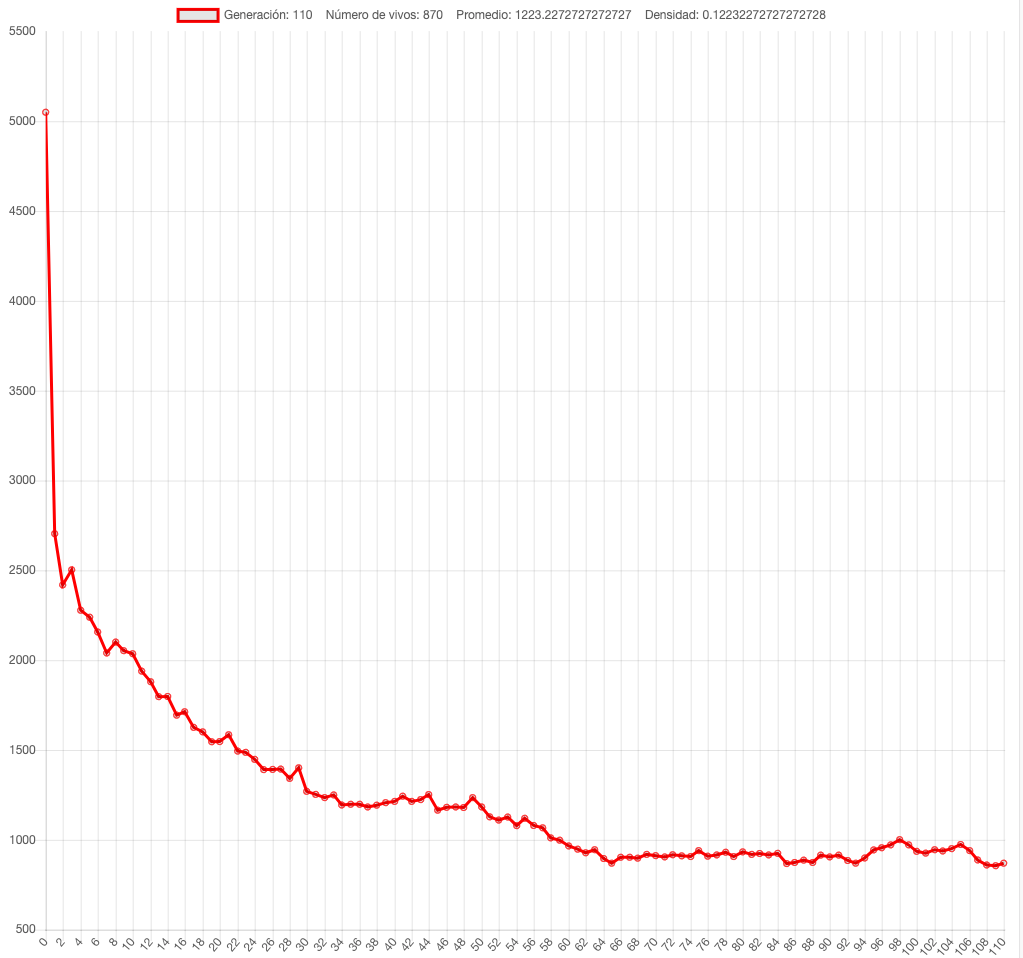
\includegraphics[scale=.24]{GOL/img/life2.png}
			\caption{Total células vivas en juego de la vida después de 100 generaciones}
			\label{fig:gol5}
		\end{center}
	\end{figure}

	\begin{figure}[H]
		\begin{center}
			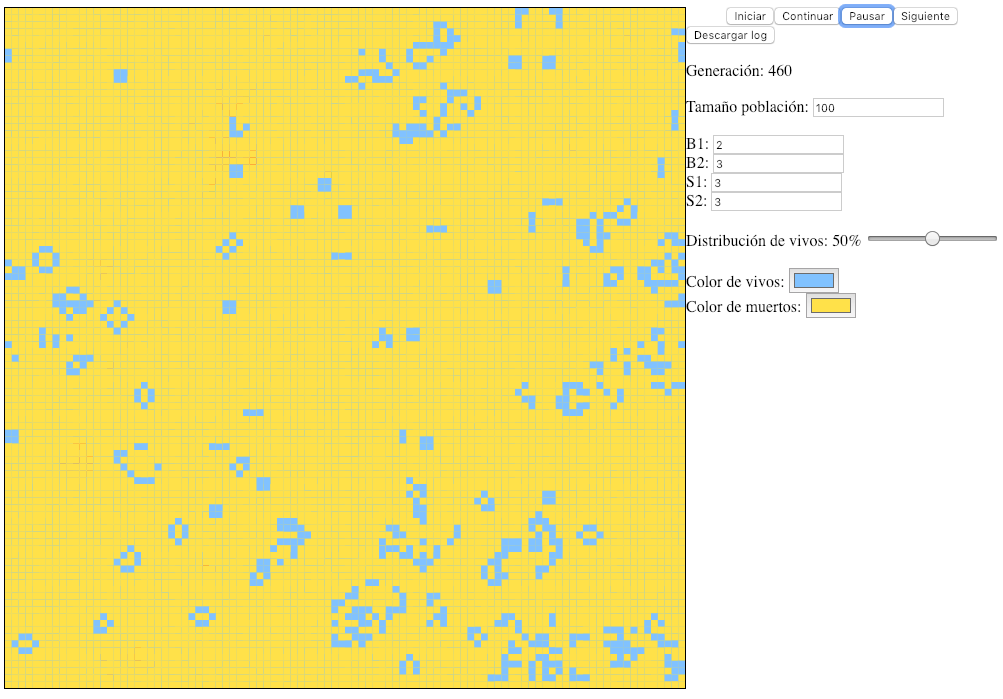
\includegraphics[scale=.3]{GOL/img/lifecolores.png}
			\caption{Juego de la vida con distintos colores}
			\label{fig:gol5}
		\end{center}
	\end{figure}

	\begin{figure}[H]
		\begin{center}
			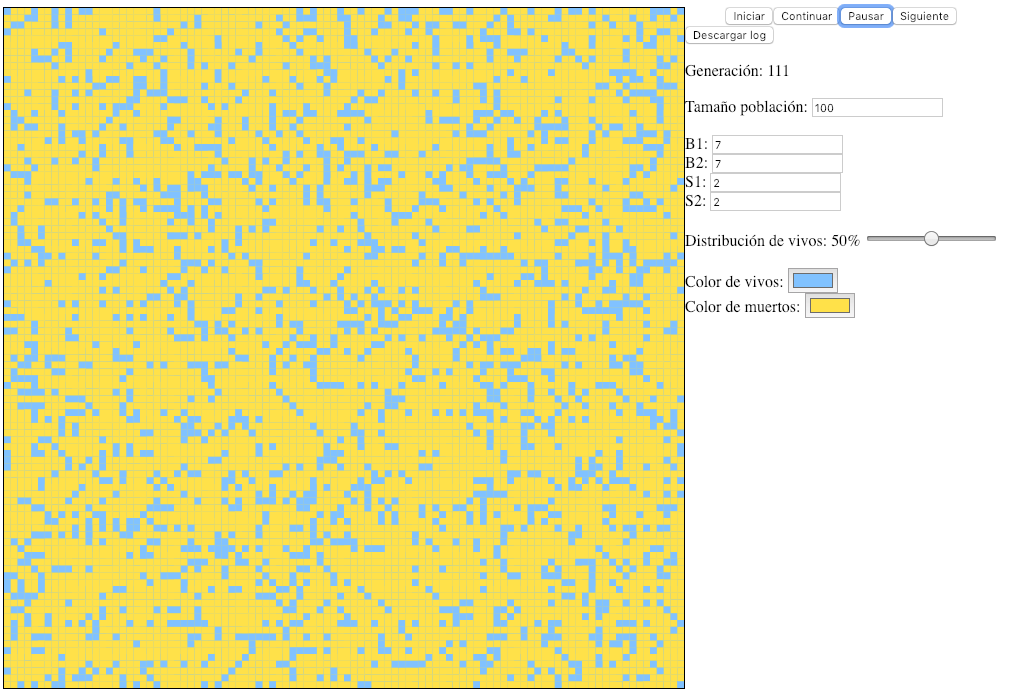
\includegraphics[scale=.3]{GOL/img/difusion1.png}
			\caption{Regla de difusión después de 100 generaciones}
			\label{fig:gol5}
		\end{center}
	\end{figure}

	\begin{figure}[H]
		\begin{center}
			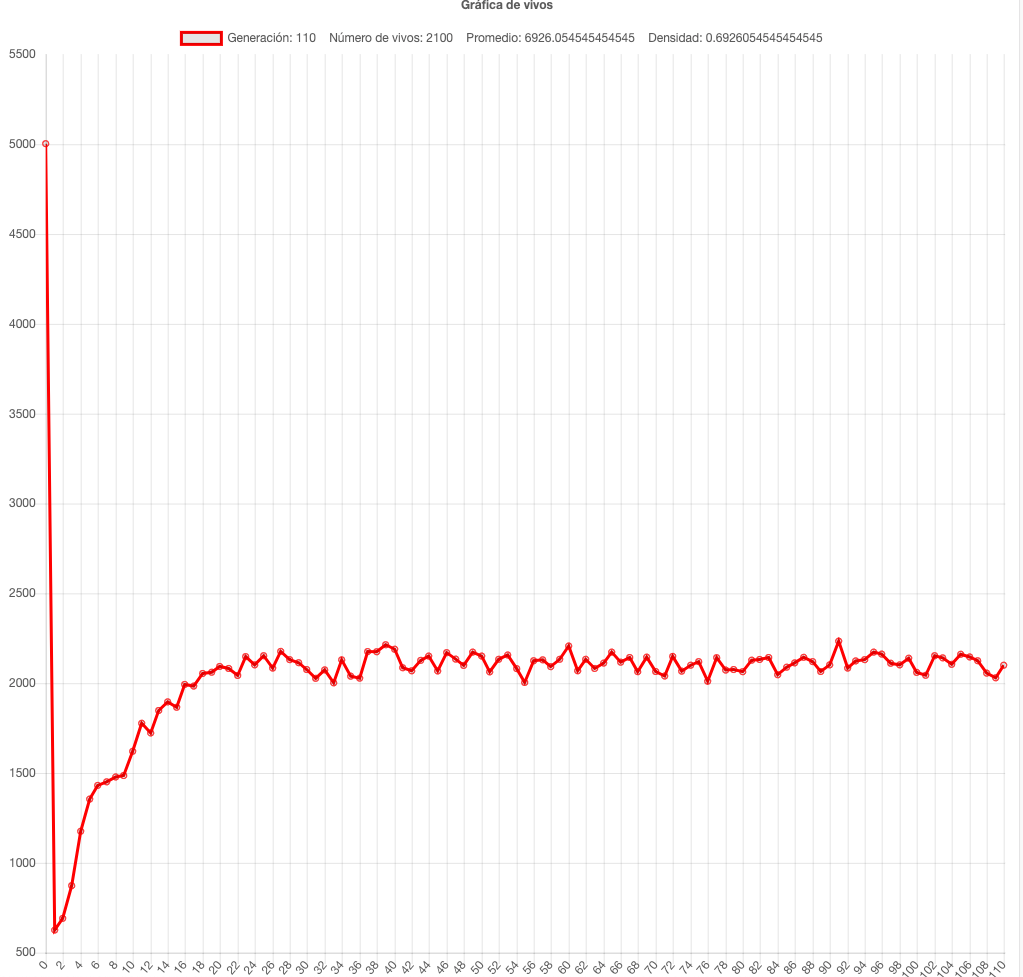
\includegraphics[scale=.24]{GOL/img/difusion2.png}
			\caption{Total células vivas con regla difusión después de 100 generaciones}
			\label{fig:gol5}
		\end{center}
	\end{figure}

\subsubsection{Análisis de poblaciones}
	En esta parte se hicieron pruebas con la regla de life y difusión aumentando la densidad de la población de 10 en 10 por ciento hasta llegar al máximo de 90 por ciento debido que en un 100 por ciento no se aprecia nada al igual que en cero, las pruebas de realizaron tras 1000 generaciones en una matriz de 100 por 100.

	\begin{figure}[H]
		\begin{center}
			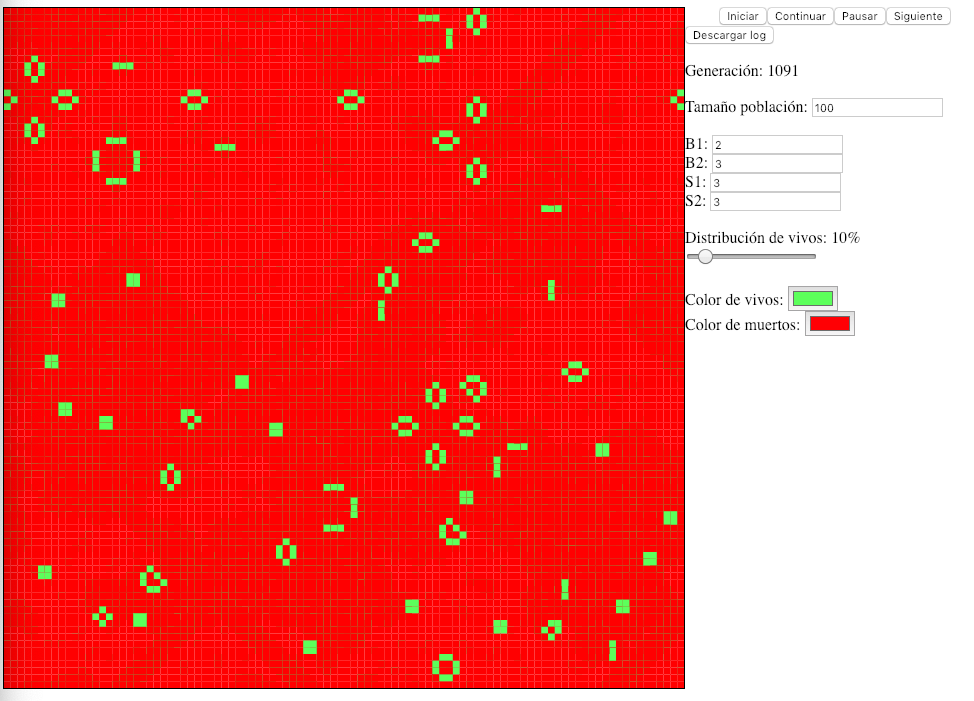
\includegraphics[scale=.3]{GOL/img/life10-1.png}
			\caption{Regla de life con probabilidad de 10\%}
			\label{fig:gol5}
		\end{center}
	\end{figure}

	\begin{figure}[H]
		\begin{center}
			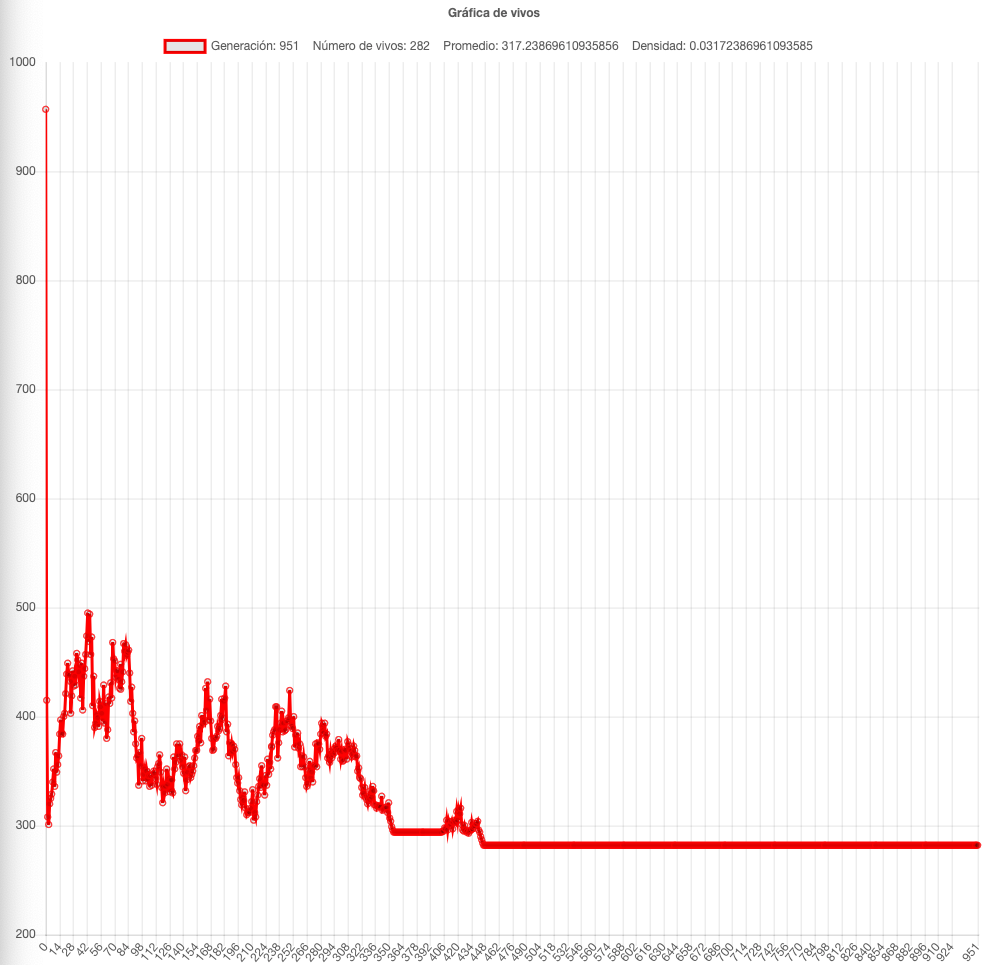
\includegraphics[scale=.24]{GOL/img/life10-2.png}
			\caption{Comportamiento de la población de la simulación anterior}
			\label{fig:gol5}
		\end{center}
	\end{figure}

	\begin{figure}[H]
		\begin{center}
			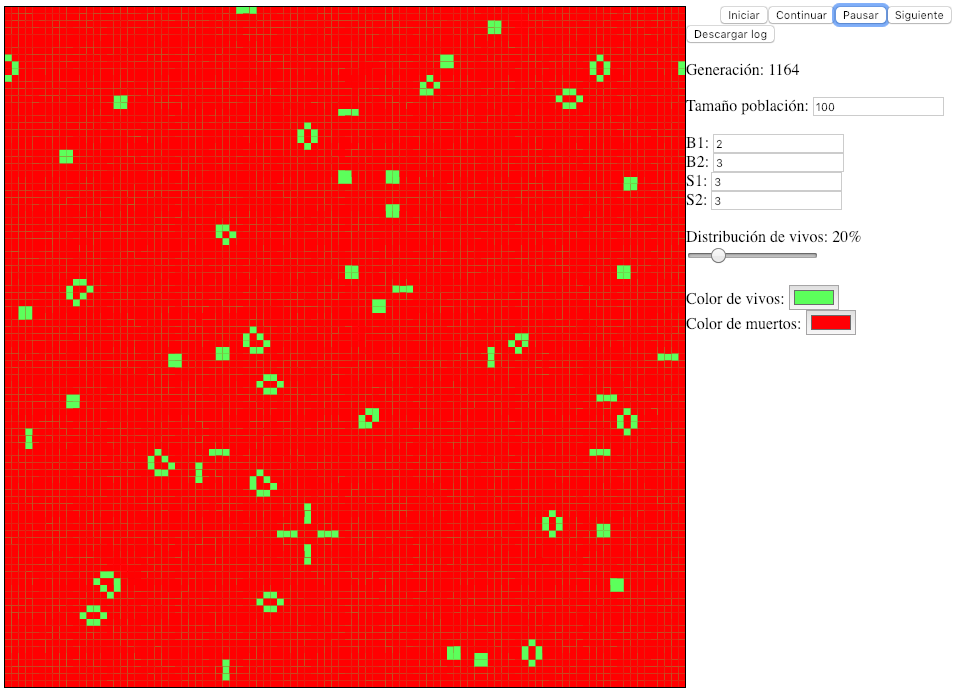
\includegraphics[scale=.3]{GOL/img/life20-1.png}
			\caption{Regla de life con probabilidad de 20\%}
			\label{fig:gol5}
		\end{center}
	\end{figure}

	\begin{figure}[H]
		\begin{center}
			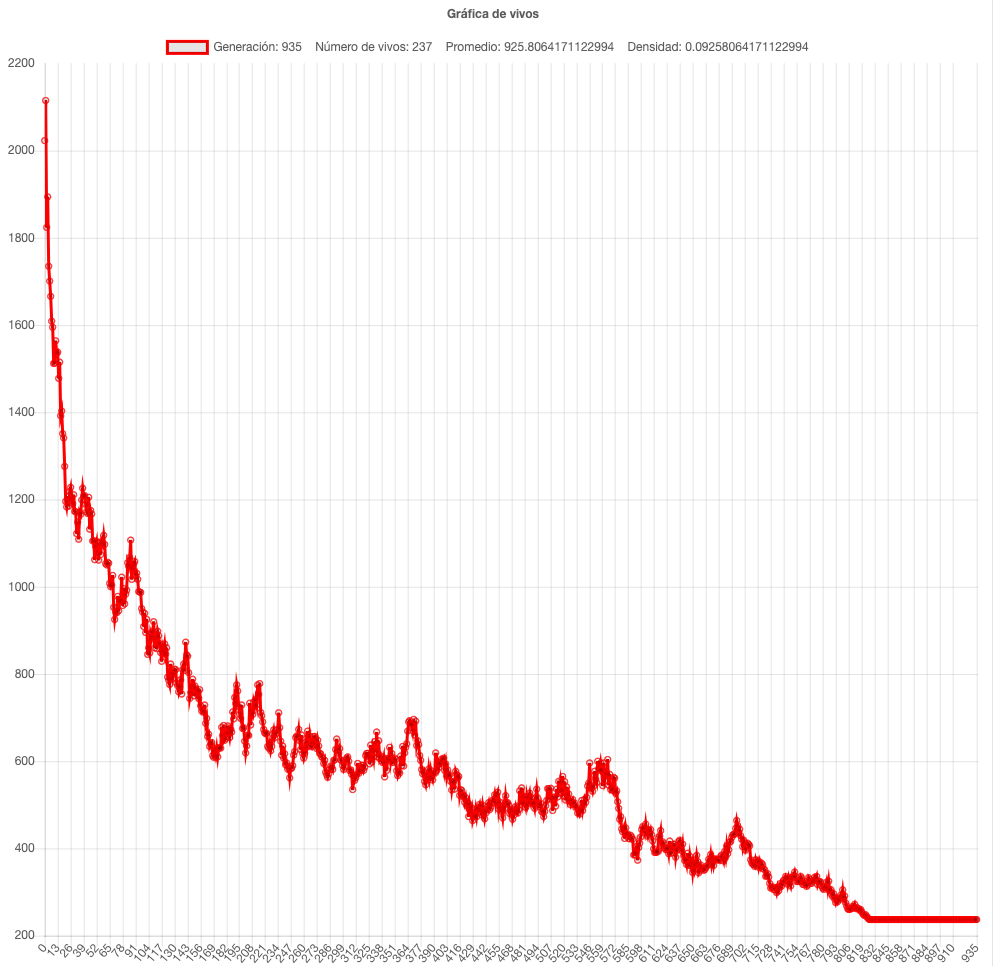
\includegraphics[scale=.24]{GOL/img/life20-2.png}
			\caption{Comportamiento de la población de la simulación anterior}
			\label{fig:gol5}
		\end{center}
	\end{figure}

	\begin{figure}[H]
		\begin{center}
			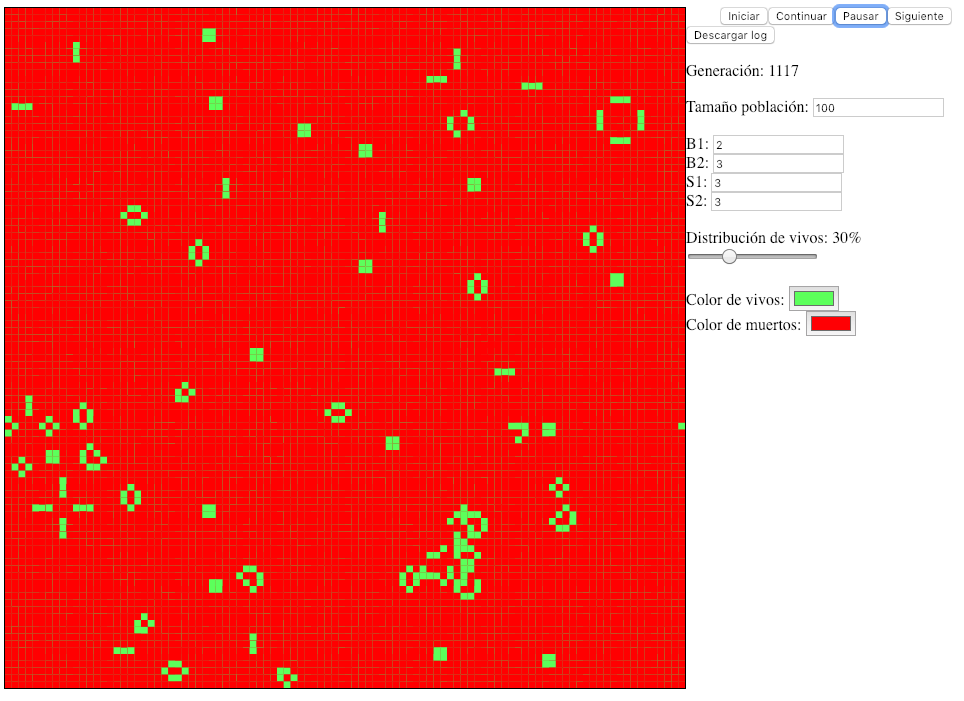
\includegraphics[scale=.3]{GOL/img/life30-1.png}
			\caption{Regla de life con probabilidad de 30\%}
			\label{fig:gol5}
		\end{center}
	\end{figure}

	\begin{figure}[H]
		\begin{center}
			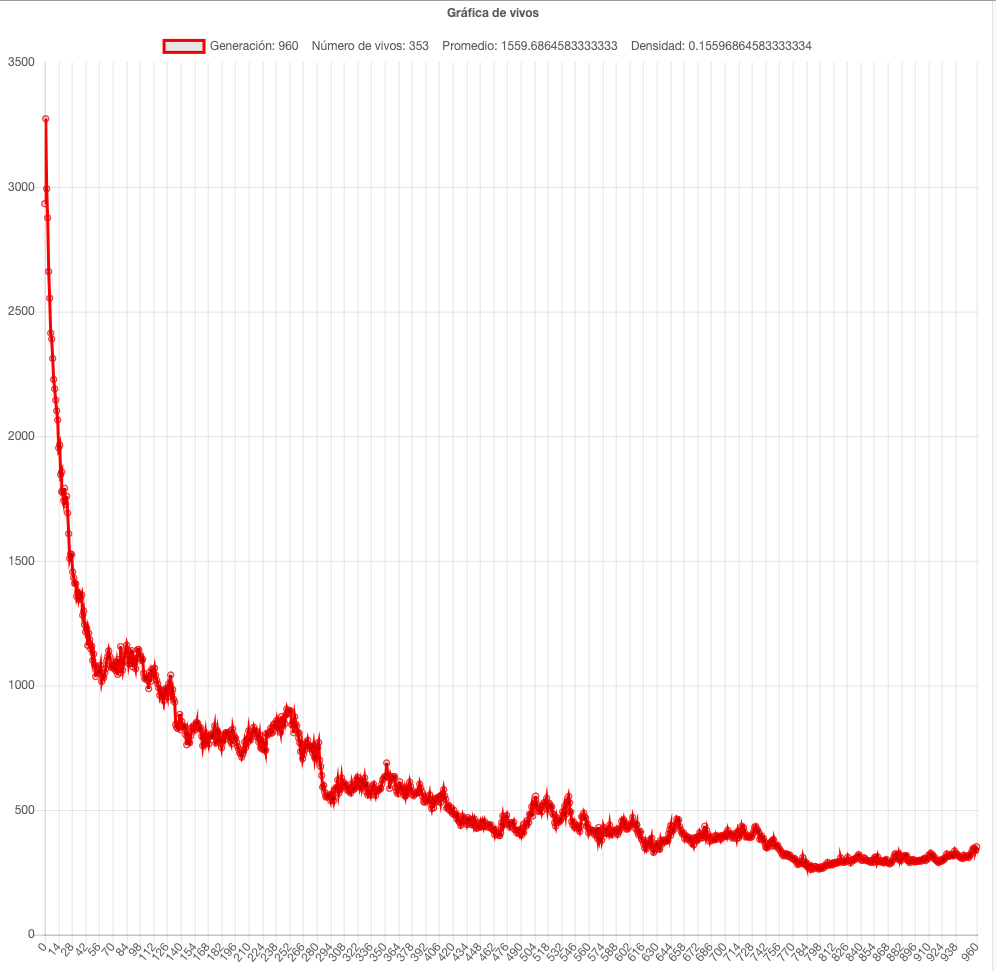
\includegraphics[scale=.24]{GOL/img/life30-2.png}
			\caption{Comportamiento de la población de la simulación anterior}
			\label{fig:gol5}
		\end{center}
	\end{figure}

	\begin{figure}[H]
		\begin{center}
			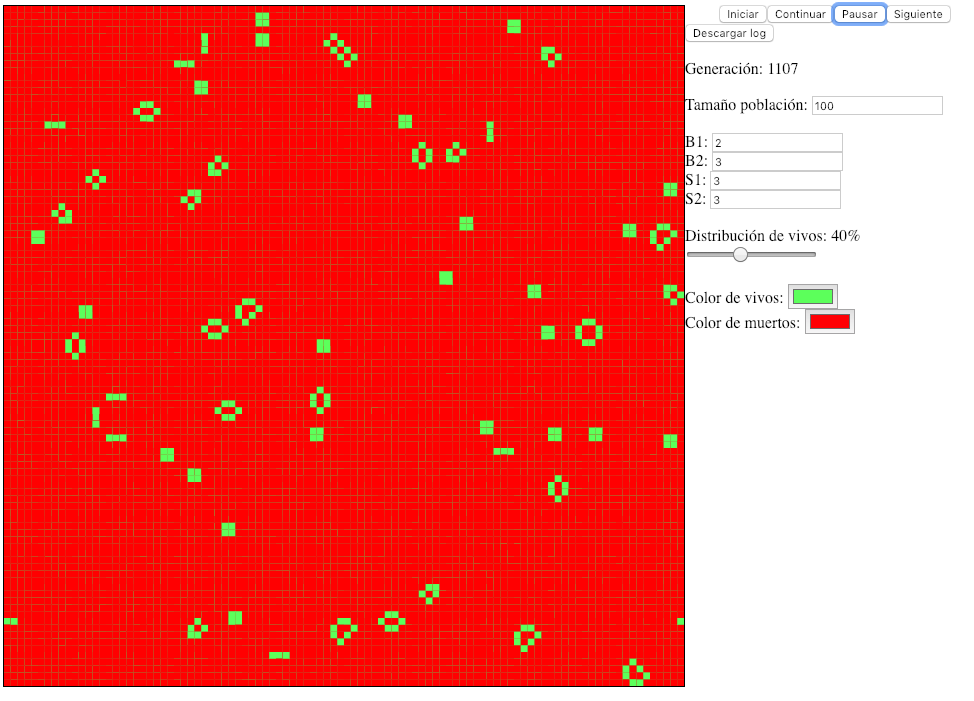
\includegraphics[scale=.3]{GOL/img/life40-1.png}
			\caption{Regla de life con probabilidad de 40\%}
			\label{fig:gol5}
		\end{center}
	\end{figure}

	\begin{figure}[H]
		\begin{center}
			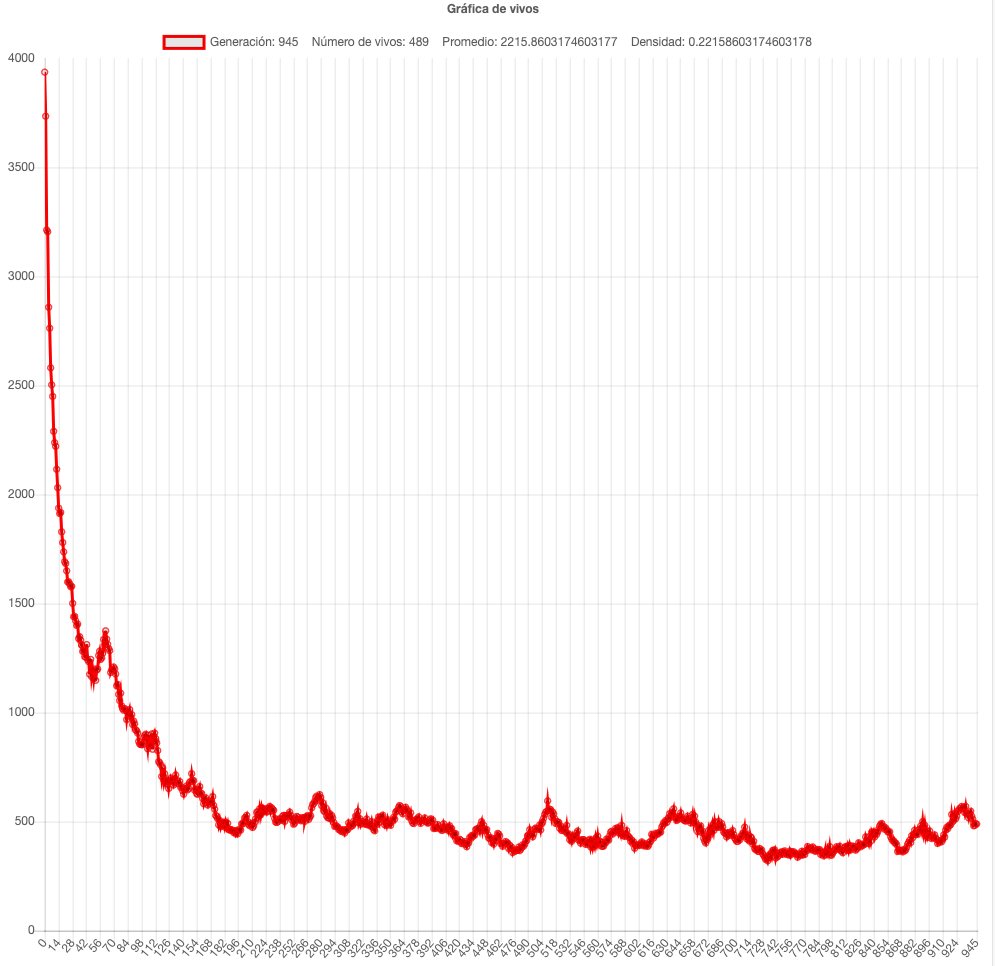
\includegraphics[scale=.24]{GOL/img/life40-2.png}
			\caption{Comportamiento de la población de la simulación anterior}
			\label{fig:gol5}
		\end{center}
	\end{figure}

	\begin{figure}[H]
		\begin{center}
			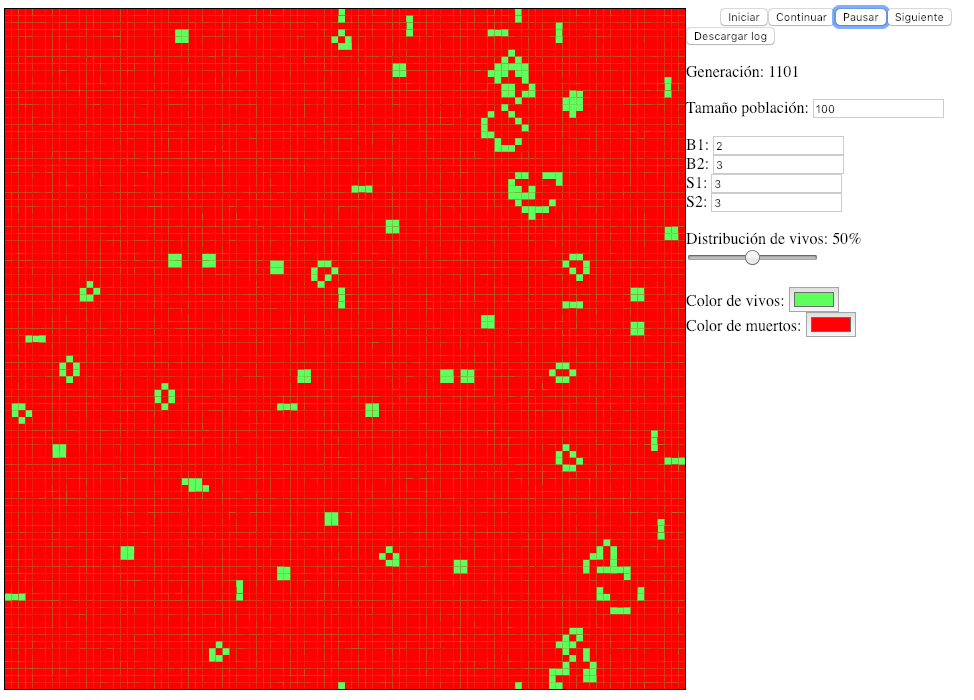
\includegraphics[scale=.3]{GOL/img/life50-1.png}
			\caption{Regla de life con probabilidad de 50\%}
			\label{fig:gol5}
		\end{center}
	\end{figure}

	\begin{figure}[H]
		\begin{center}
			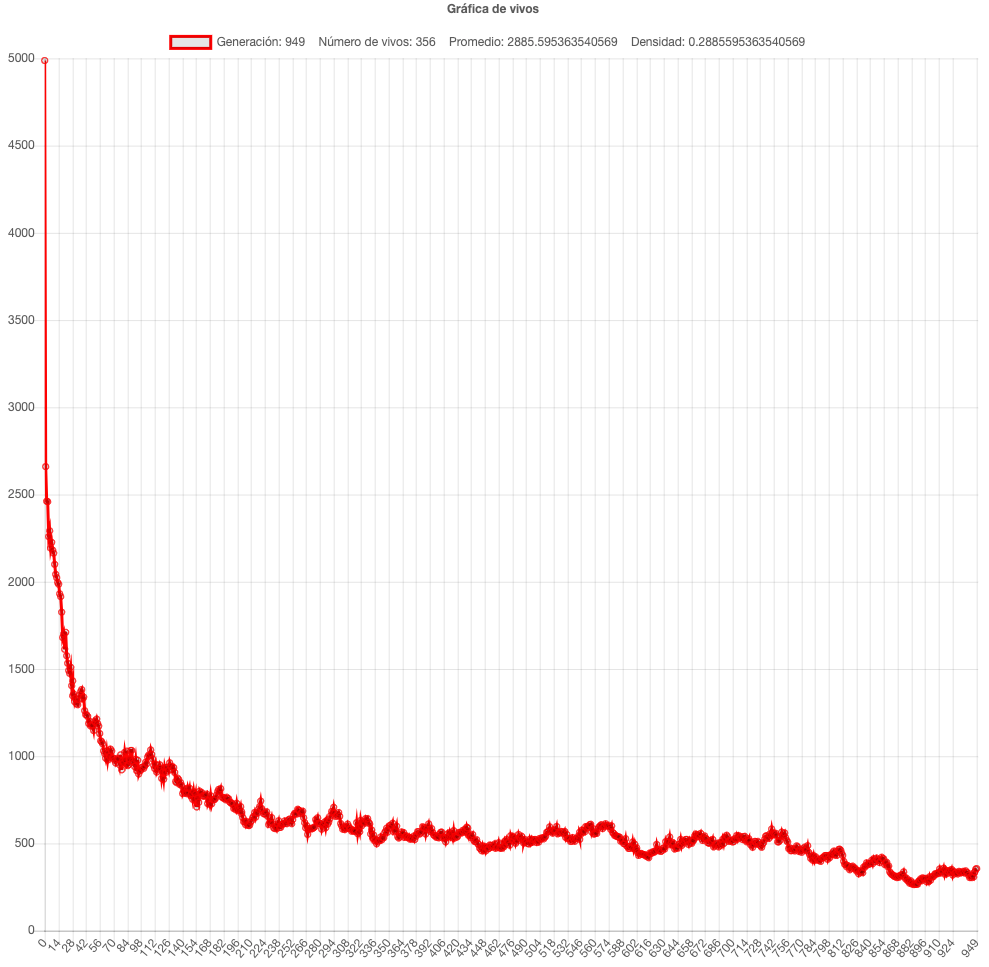
\includegraphics[scale=.24]{GOL/img/life50-2.png}
			\caption{Comportamiento de la población de la simulación anterior}
			\label{fig:gol5}
		\end{center}
	\end{figure}

	\begin{figure}[H]
		\begin{center}
			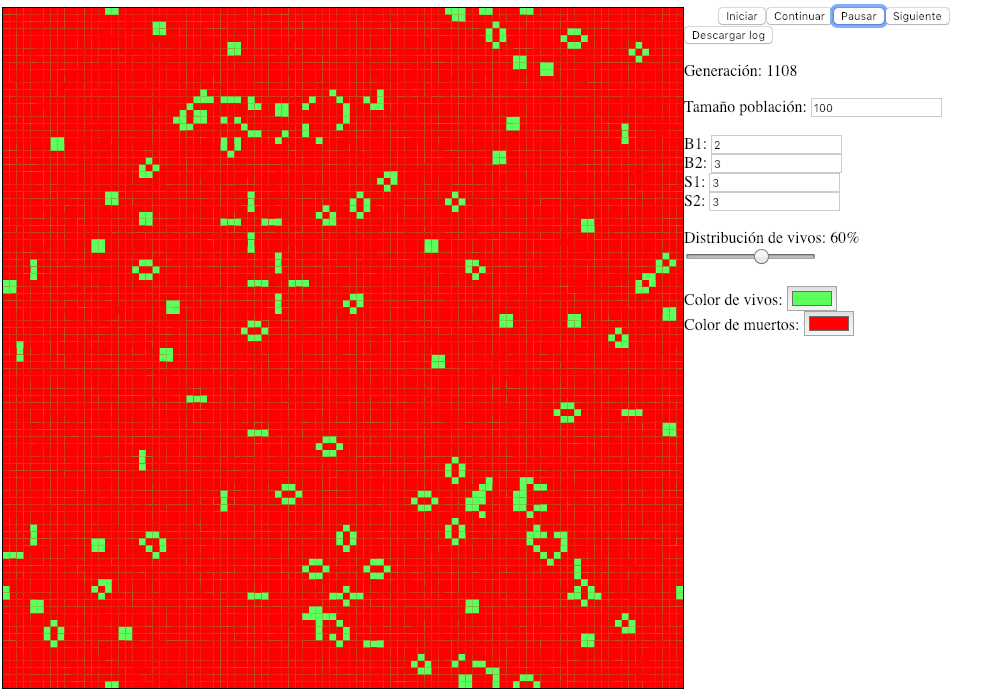
\includegraphics[scale=.3]{GOL/img/life60-1.png}
			\caption{Regla de life con probabilidad de 60\%}
			\label{fig:gol5}
		\end{center}
	\end{figure}

	\begin{figure}[H]
		\begin{center}
			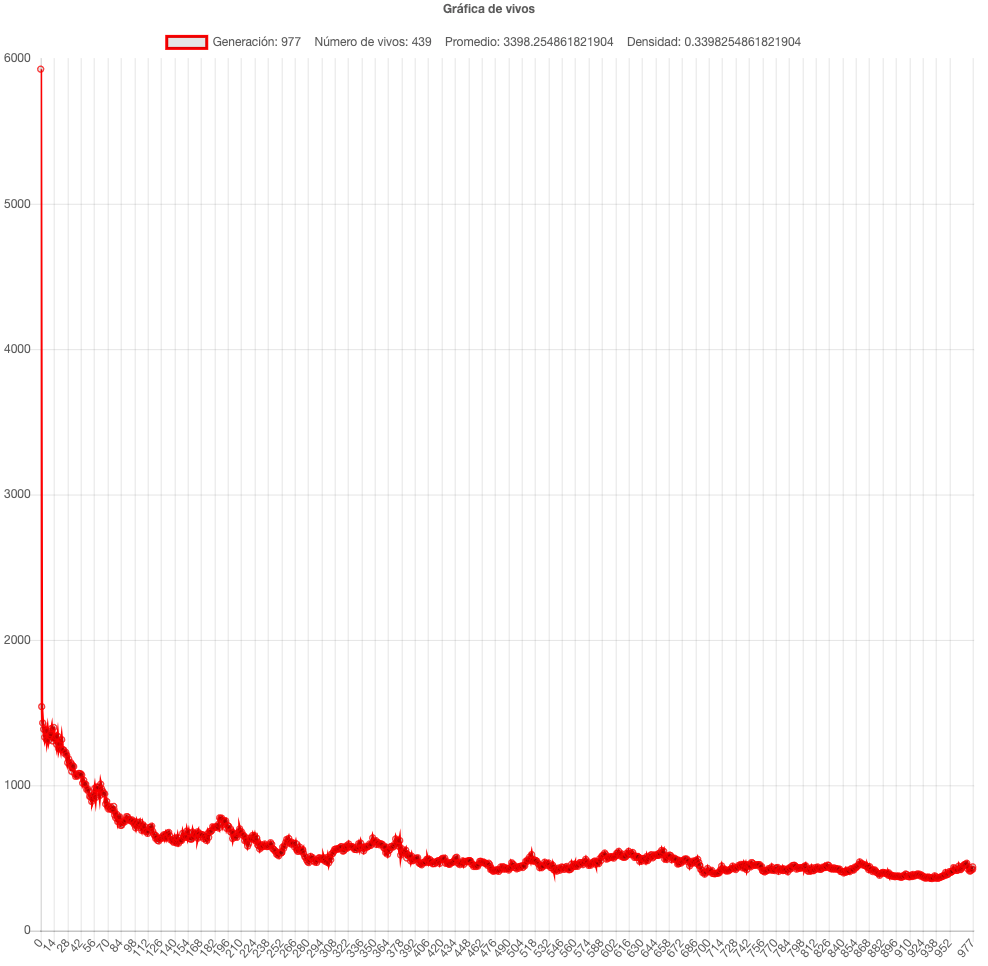
\includegraphics[scale=.24]{GOL/img/life60-2.png}
			\caption{Comportamiento de la población de la simulación anterior}
			\label{fig:gol5}
		\end{center}
	\end{figure}

	\begin{figure}[H]
		\begin{center}
			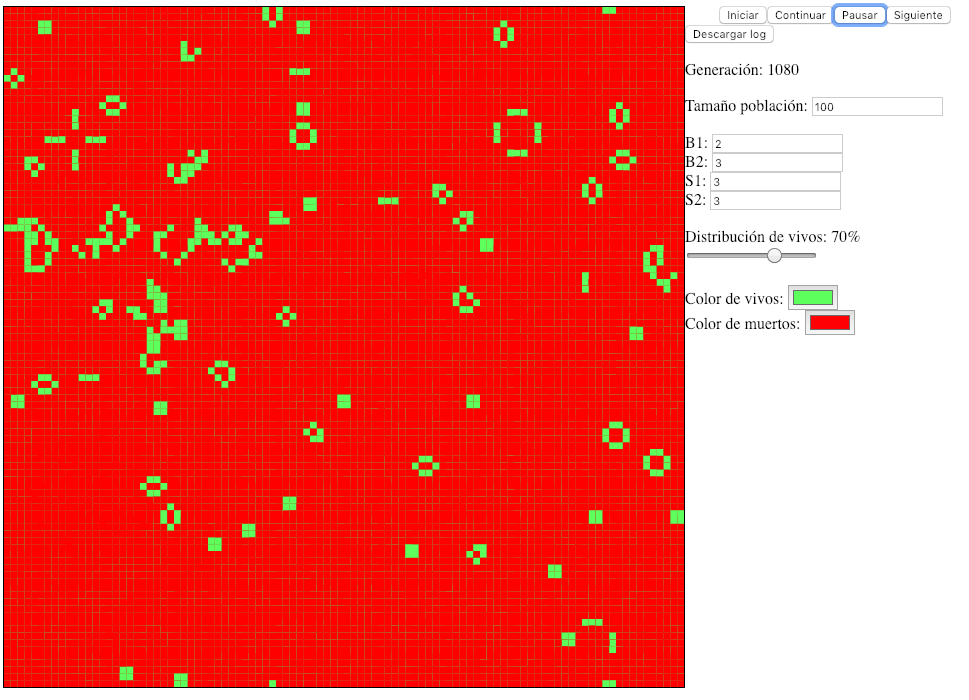
\includegraphics[scale=.3]{GOL/img/life70-1.png}
			\caption{Regla de life con probabilidad de 70\%}
			\label{fig:gol5}
		\end{center}
	\end{figure}

	\begin{figure}[H]
		\begin{center}
			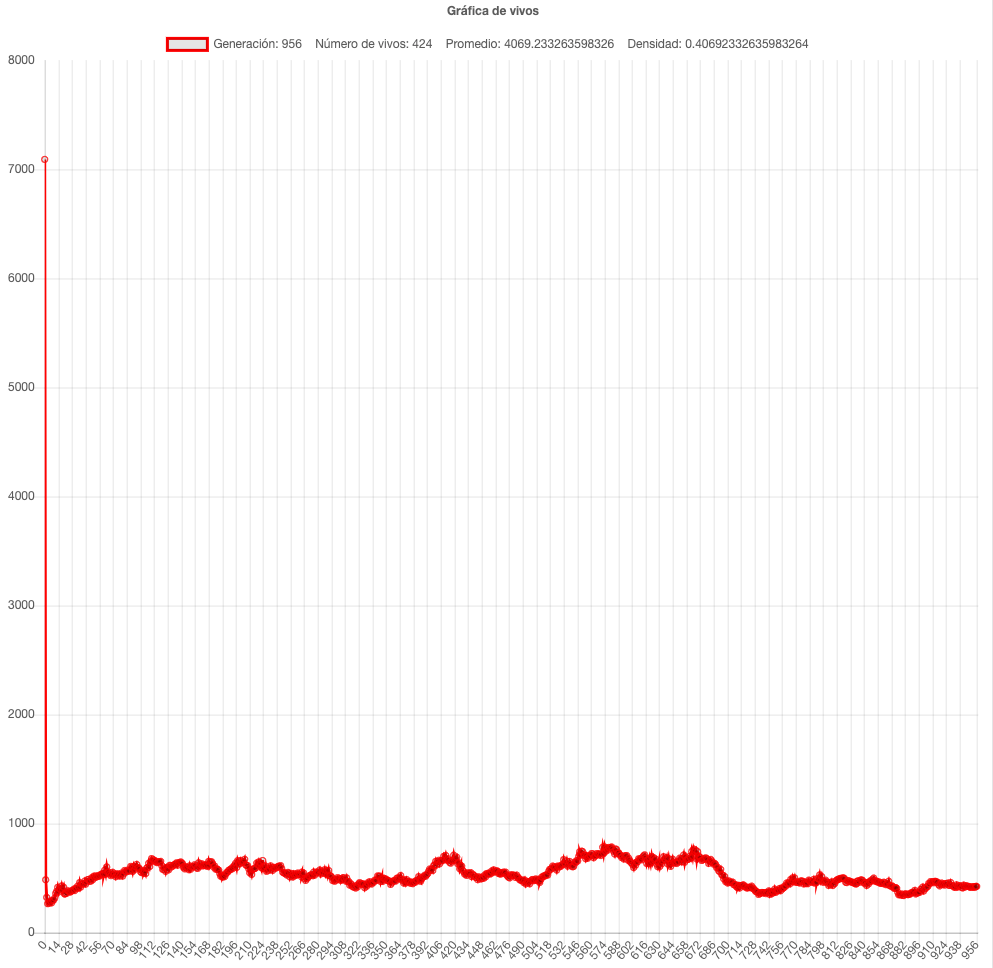
\includegraphics[scale=.24]{GOL/img/life70-2.png}
			\caption{Comportamiento de la población de la simulación anterior}
			\label{fig:gol5}
		\end{center}
	\end{figure}

	\begin{figure}[H]
		\begin{center}
			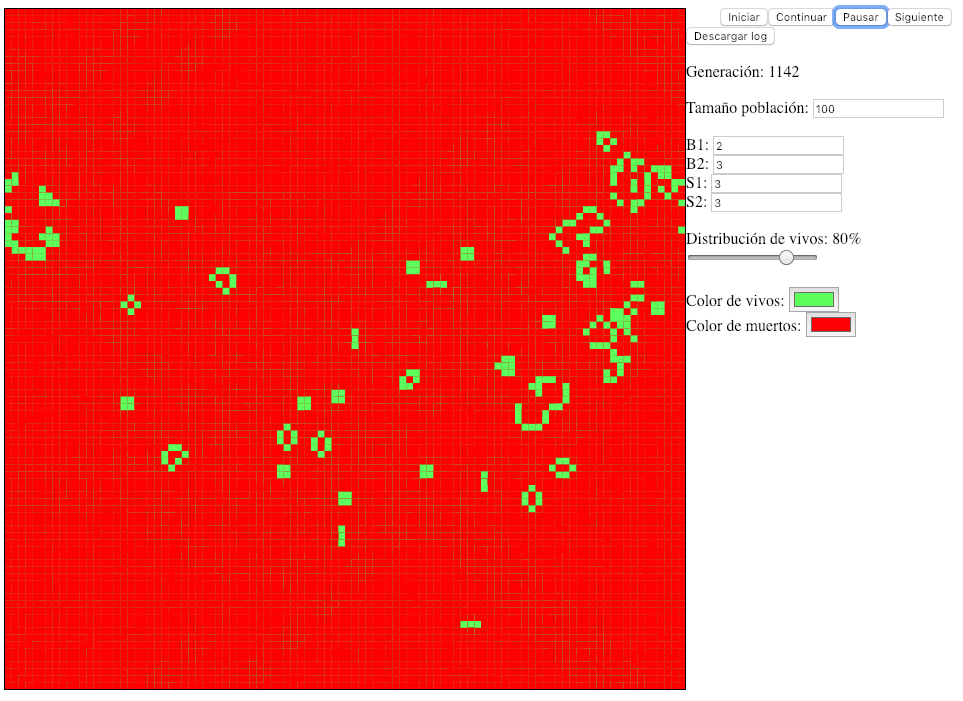
\includegraphics[scale=.3]{GOL/img/life80-1.png}
			\caption{Regla de life con probabilidad de 80\%}
			\label{fig:gol5}
		\end{center}
	\end{figure}

	\begin{figure}[H]
		\begin{center}
			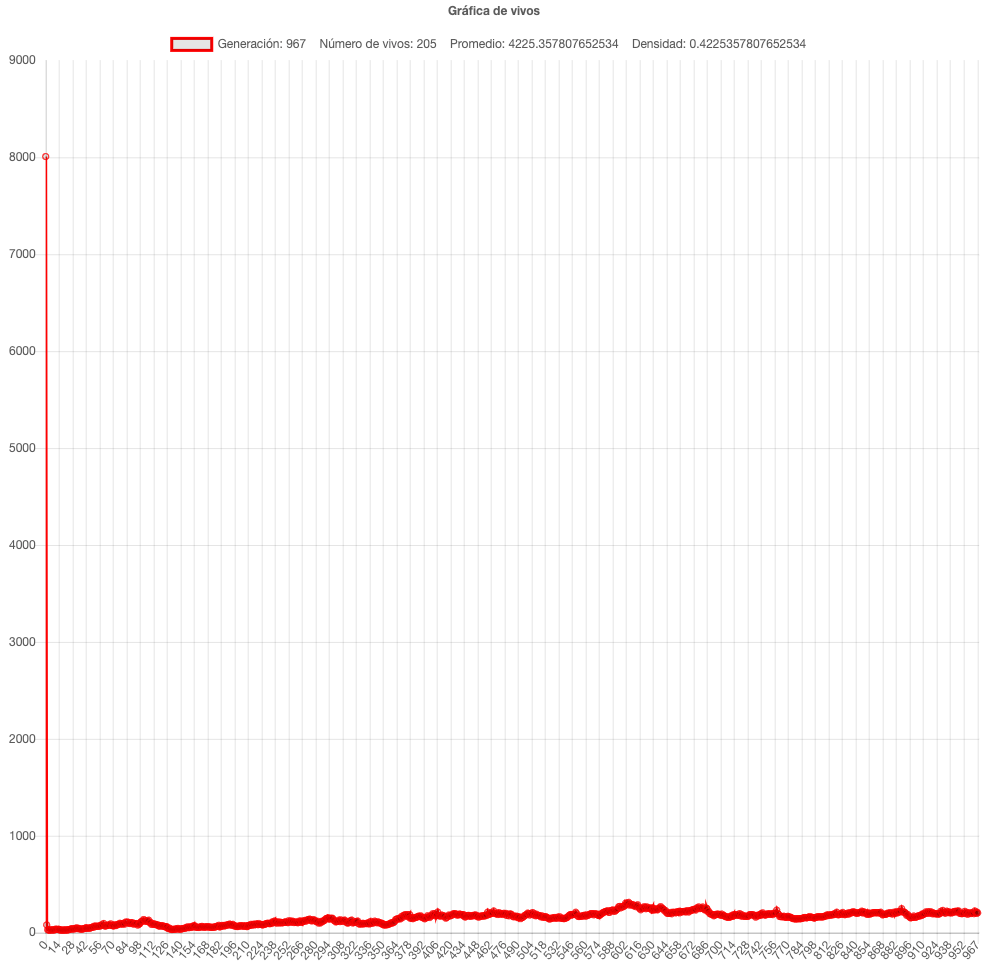
\includegraphics[scale=.24]{GOL/img/life80-2.png}
			\caption{Comportamiento de la población de la simulación anterior}
			\label{fig:gol5}
		\end{center}
	\end{figure}

	\begin{figure}[H]
		\begin{center}
			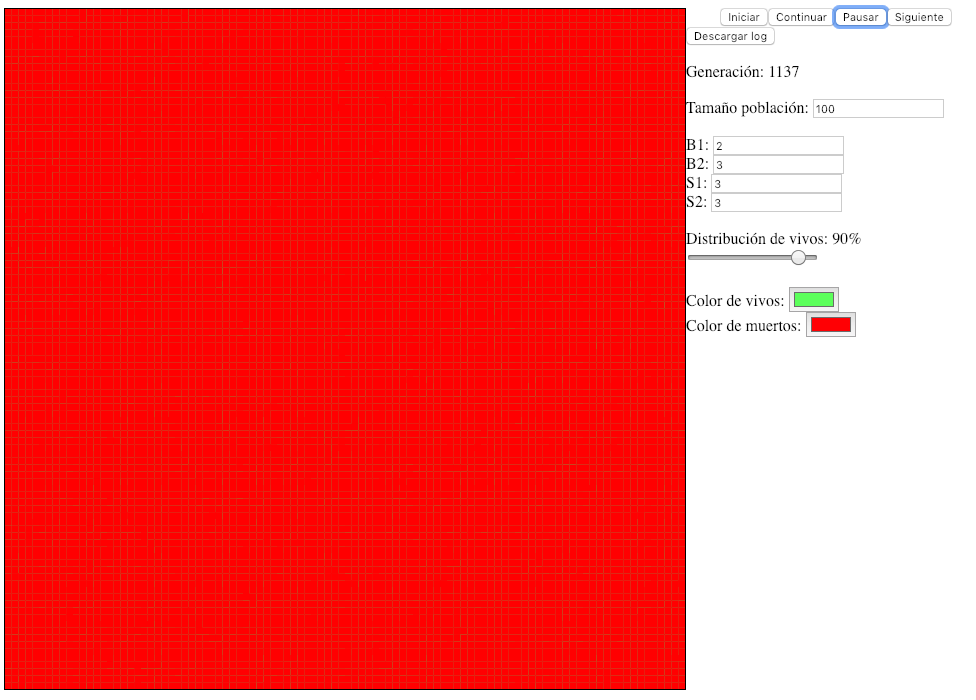
\includegraphics[scale=.3]{GOL/img/life90-1.png}
			\caption{Regla de life con probabilidad de 90\%}
			\label{fig:gol5}
		\end{center}
	\end{figure}

	\begin{figure}[H]
		\begin{center}
			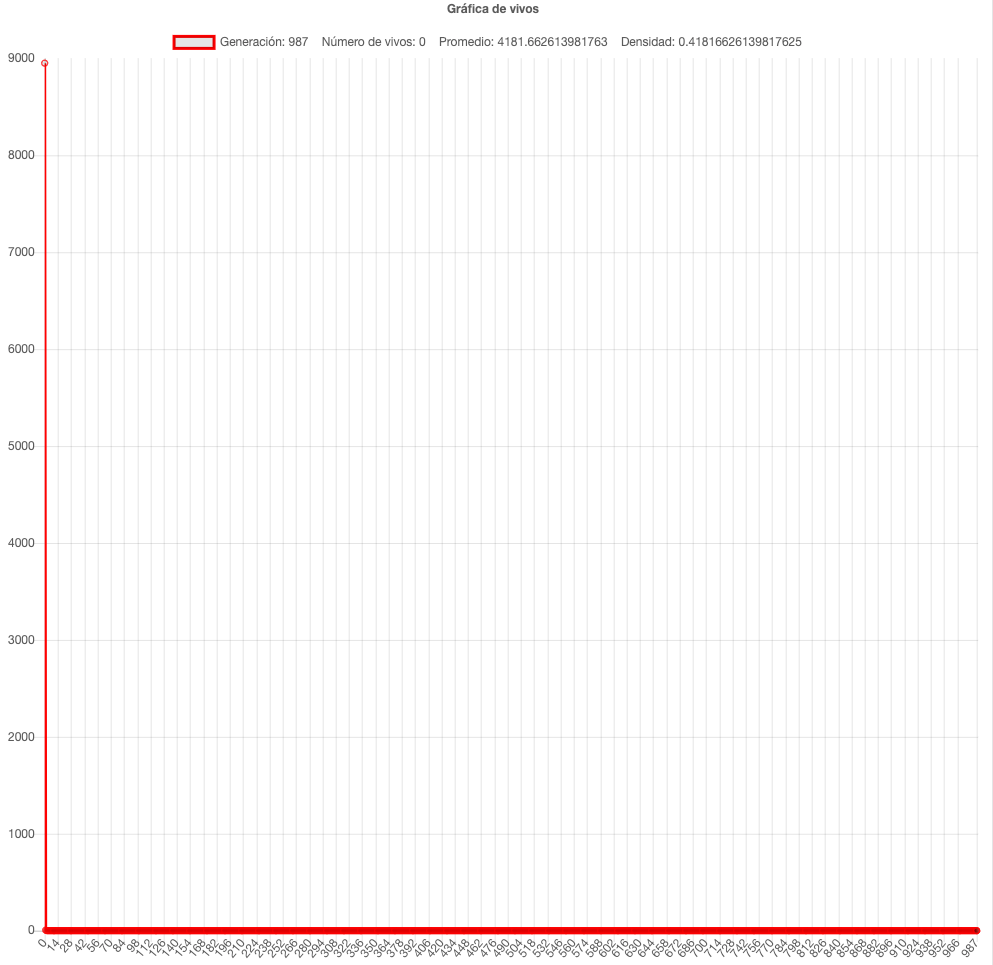
\includegraphics[scale=.24]{GOL/img/life90-2.png}
			\caption{Comportamiento de la población de la simulación anterior}
			\label{fig:gol5}
		\end{center}
	\end{figure}

	En todas las simulaciones se encuentra un comportamiento similar en el cual la población inicial es muy alta y de manera brusca disminuye y apartir de ahí decrece de manera lenta. En general, le regla de life hace que las poblaciones tiendan a una densidad de .03.

	\begin{figure}[H]
		\begin{center}
			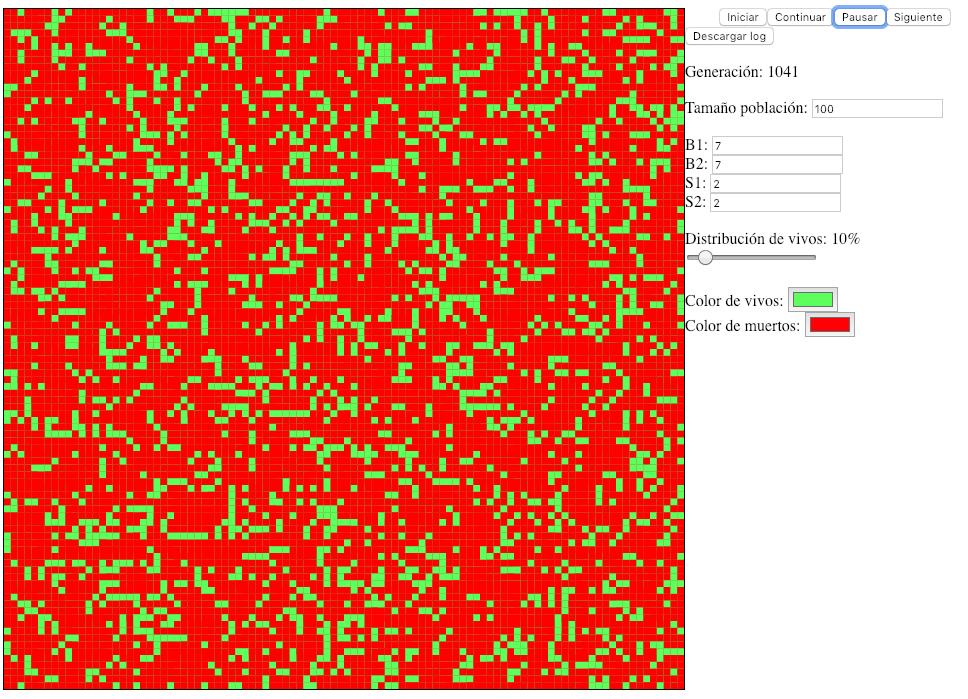
\includegraphics[scale=.3]{GOL/img/dif10-1.png}
			\caption{Regla de difusión con probabilidad de 10\%}
			\label{fig:gol5}
		\end{center}
	\end{figure}

	\begin{figure}[H]
		\begin{center}
			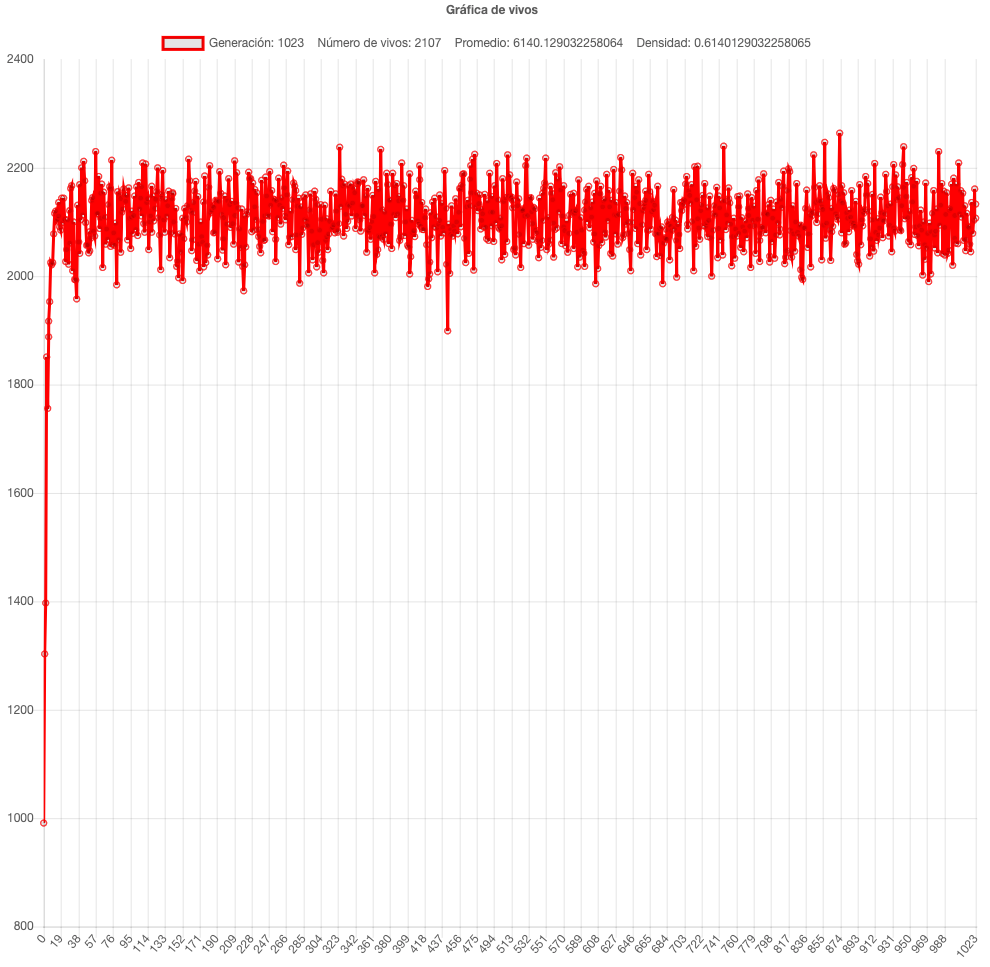
\includegraphics[scale=.24]{GOL/img/dif10-2.png}
			\caption{Comportamiento de la población de la simulación anterior}
			\label{fig:gol5}
		\end{center}
	\end{figure}

	\begin{figure}[H]
		\begin{center}
			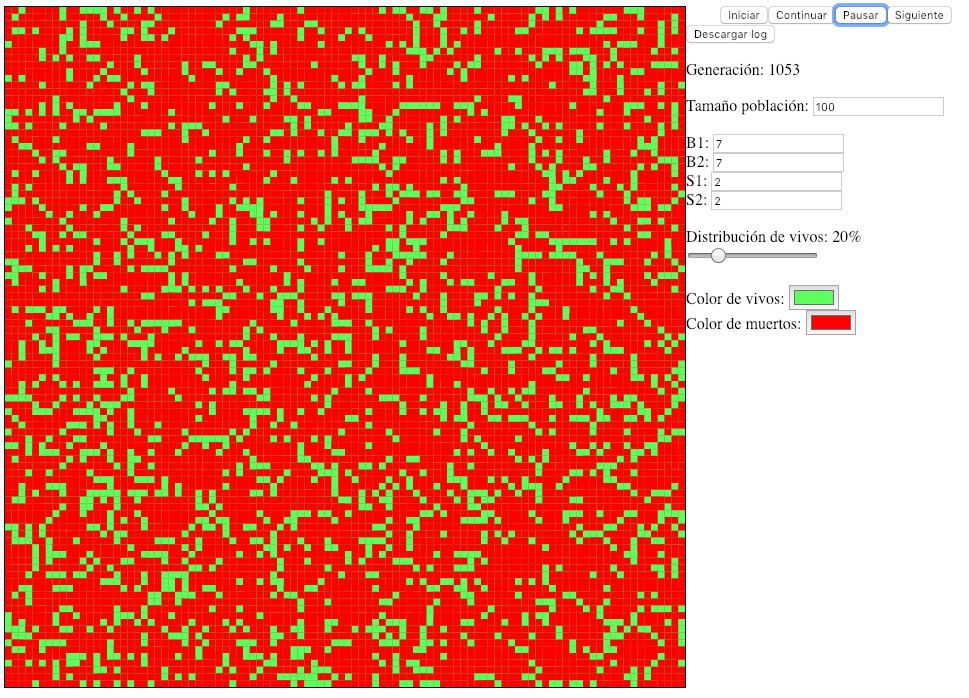
\includegraphics[scale=.3]{GOL/img/dif20-1.png}
			\caption{Regla de difusión con probabilidad de 20\%}
			\label{fig:gol5}
		\end{center}
	\end{figure}

	\begin{figure}[H]
		\begin{center}
			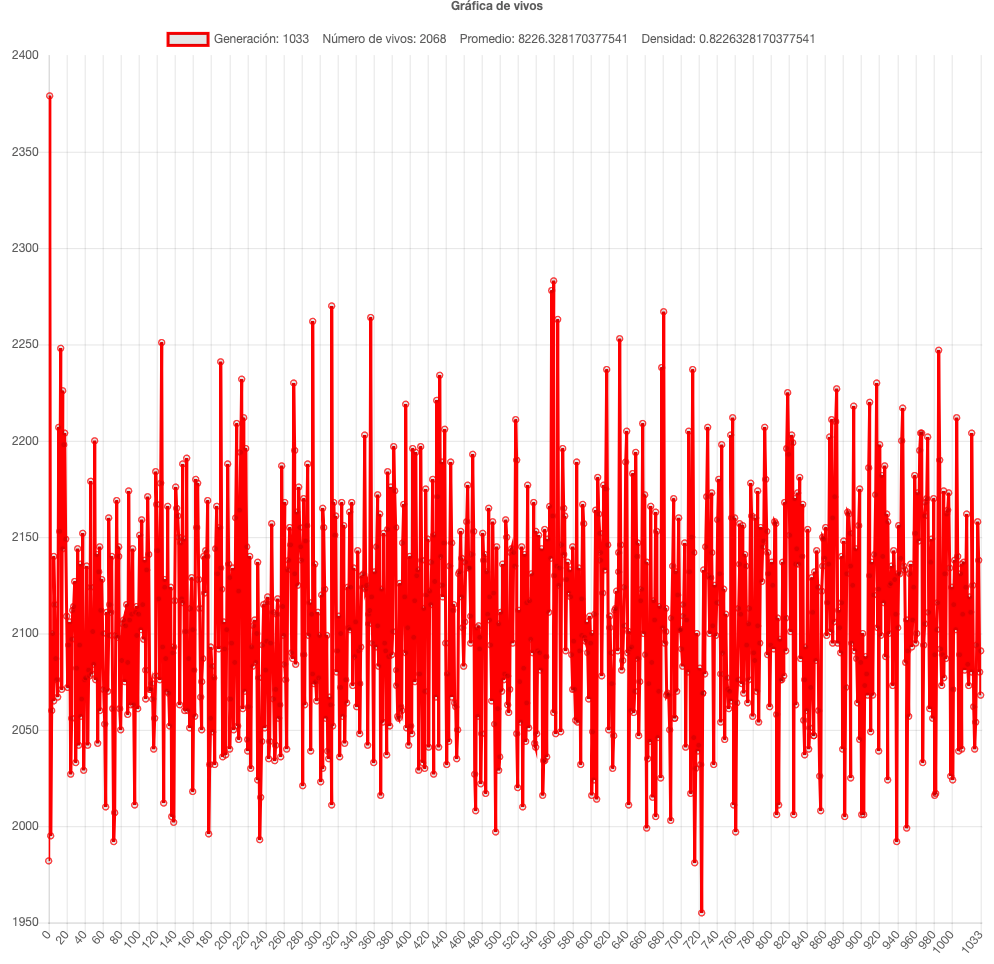
\includegraphics[scale=.24]{GOL/img/dif20-2.png}
			\caption{Comportamiento de la población de la simulación anterior}
			\label{fig:gol5}
		\end{center}
	\end{figure}

	\begin{figure}[H]
		\begin{center}
			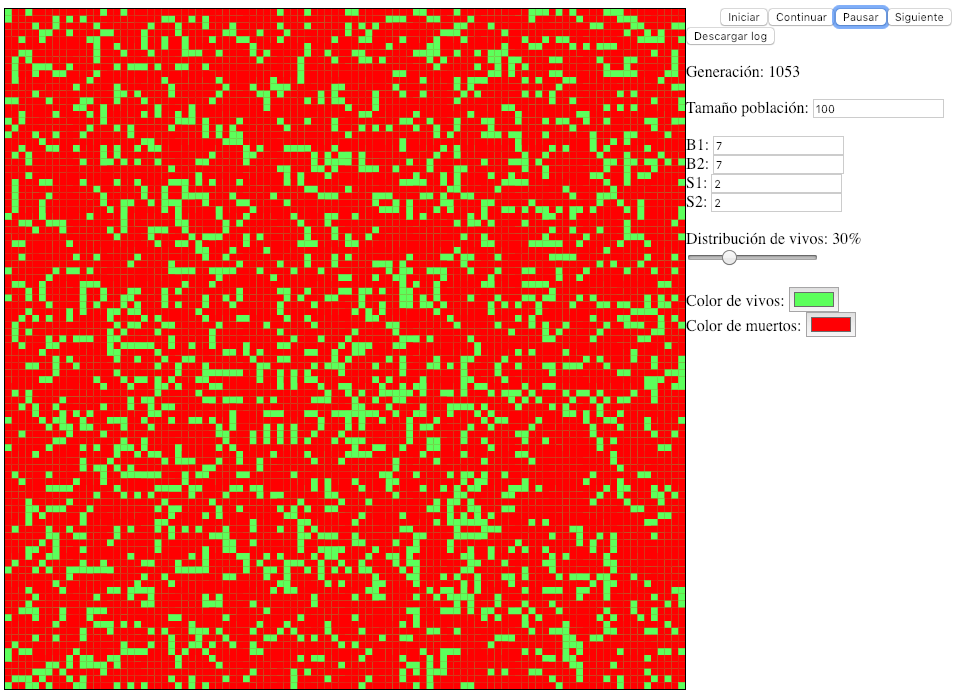
\includegraphics[scale=.3]{GOL/img/dif30-1.png}
			\caption{Regla de difusión con probabilidad de 30\%}
			\label{fig:gol5}
		\end{center}
	\end{figure}

	\begin{figure}[H]
		\begin{center}
			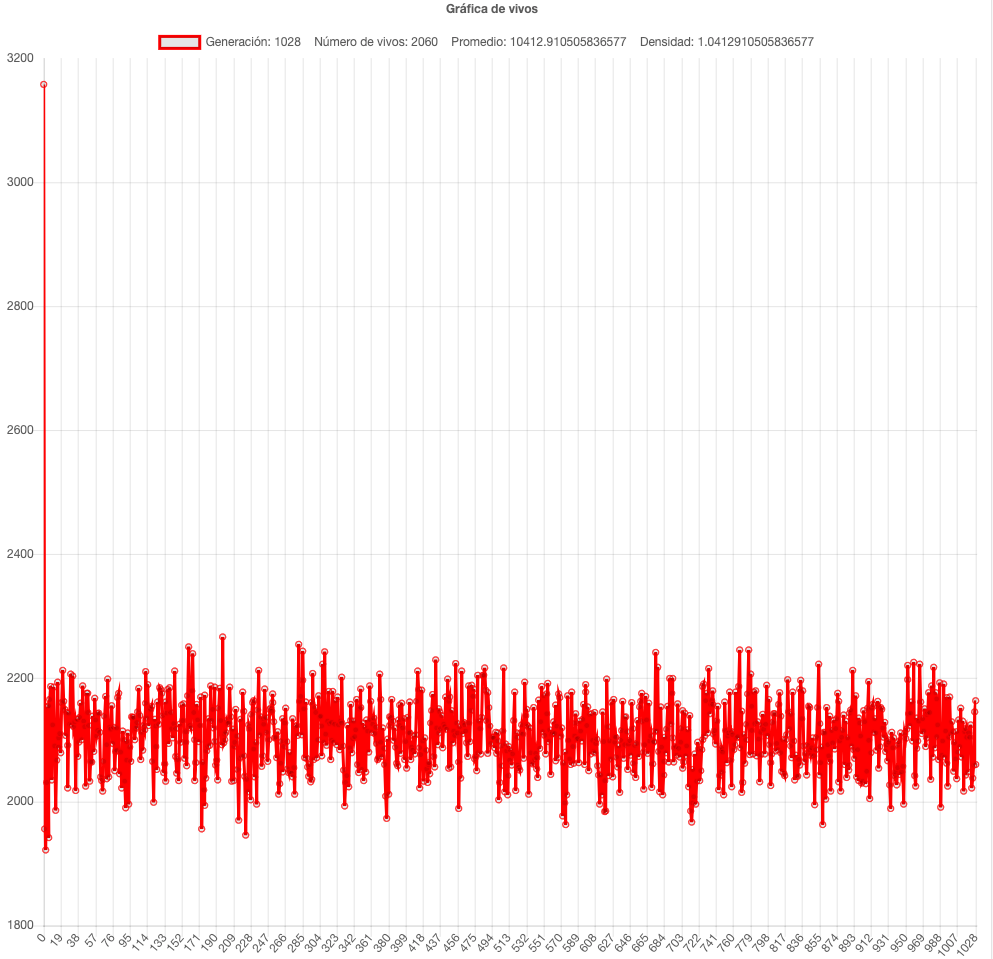
\includegraphics[scale=.24]{GOL/img/dif30-2.png}
			\caption{Comportamiento de la población de la simulación anterior}
			\label{fig:gol5}
		\end{center}
	\end{figure}

	\begin{figure}[H]
		\begin{center}
			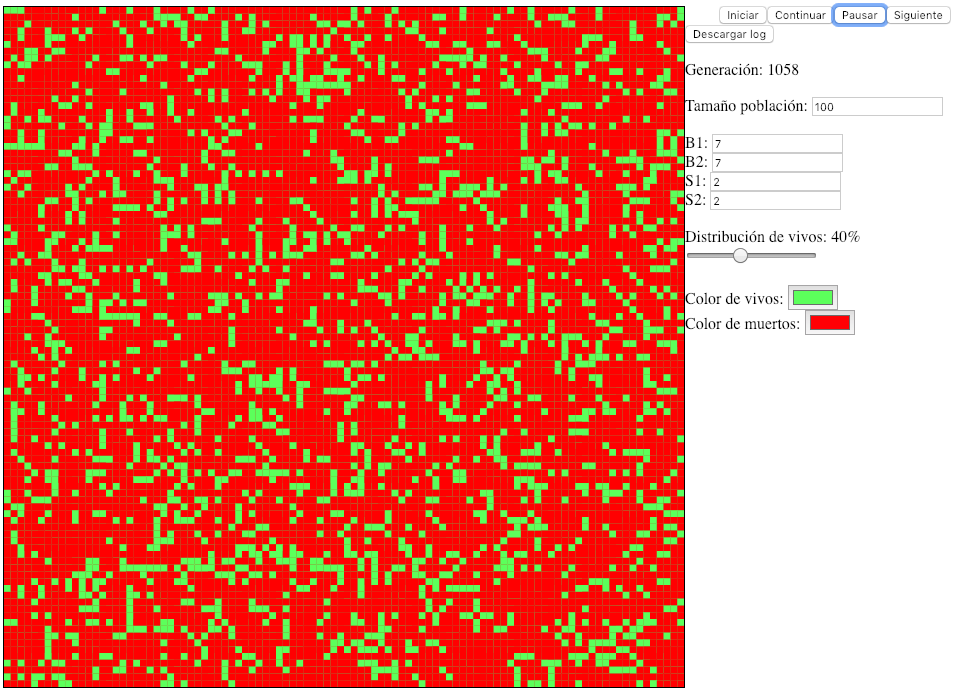
\includegraphics[scale=.3]{GOL/img/dif40-1.png}
			\caption{Regla de difusión con probabilidad de 40\%}
			\label{fig:gol5}
		\end{center}
	\end{figure}

	\begin{figure}[H]
		\begin{center}
			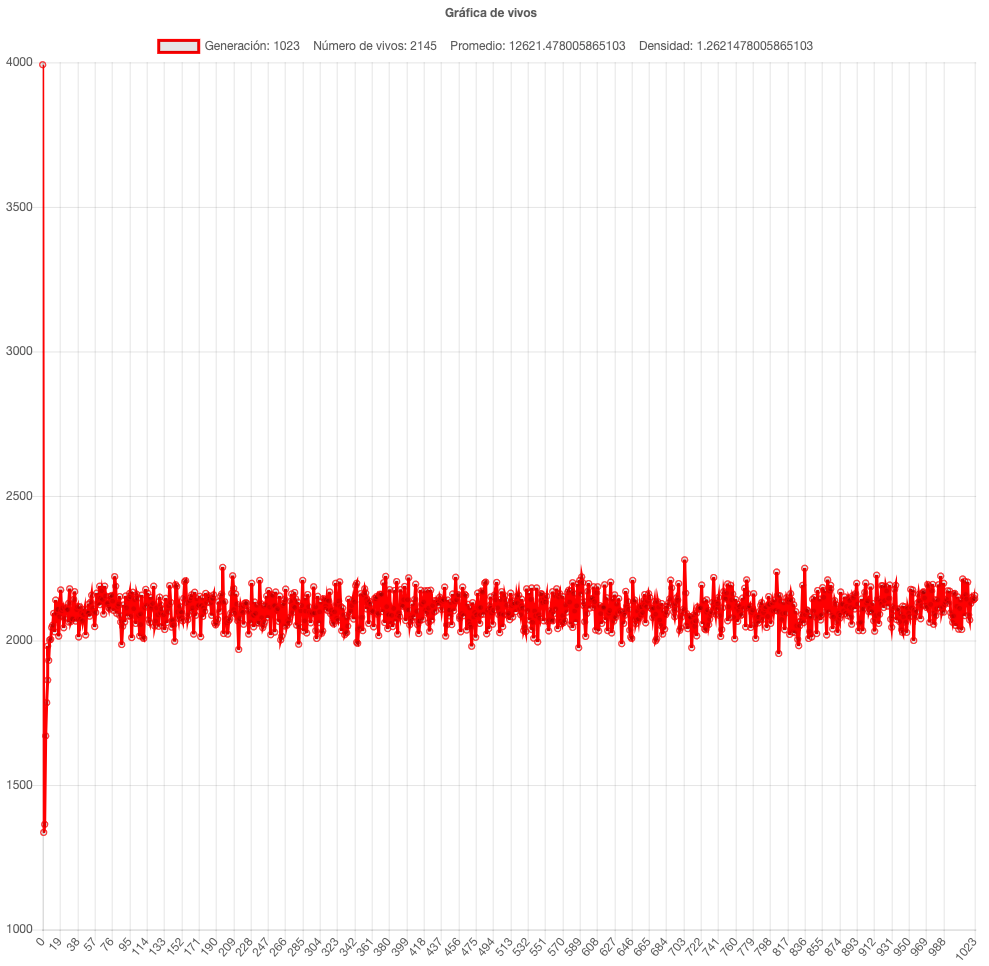
\includegraphics[scale=.24]{GOL/img/dif40-2.png}
			\caption{Comportamiento de la población de la simulación anterior}
			\label{fig:gol5}
		\end{center}
	\end{figure}

	\begin{figure}[H]
		\begin{center}
			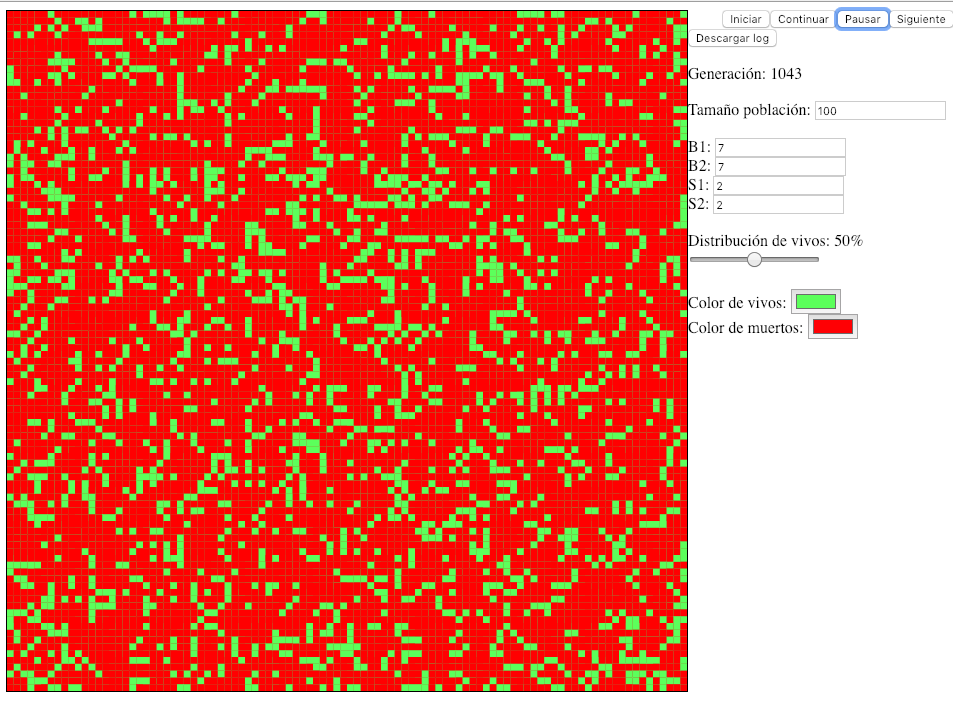
\includegraphics[scale=.3]{GOL/img/dif50-1.png}
			\caption{Regla de difusión con probabilidad de 50\%}
			\label{fig:gol5}
		\end{center}
	\end{figure}

	\begin{figure}[H]
		\begin{center}
			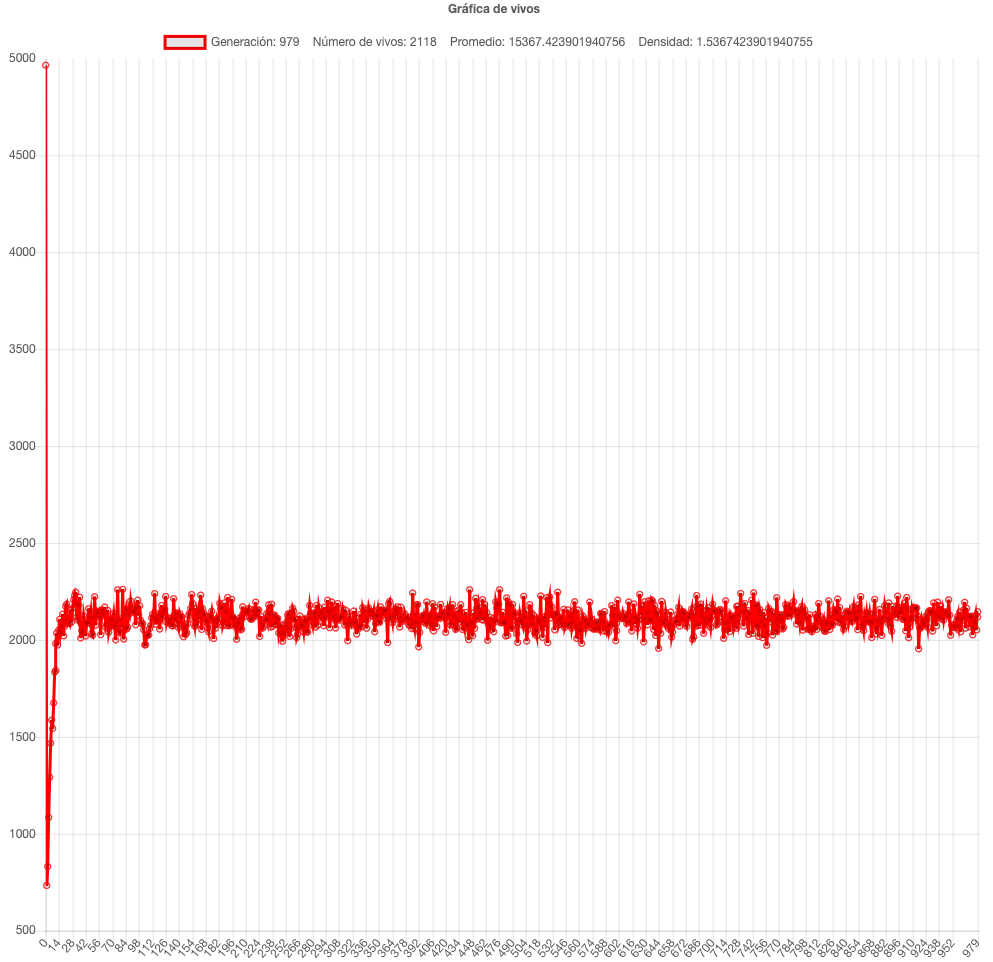
\includegraphics[scale=.24]{GOL/img/dif50-2.png}
			\caption{Comportamiento de la población de la simulación anterior}
			\label{fig:gol5}
		\end{center}
	\end{figure}

	\begin{figure}[H]
		\begin{center}
			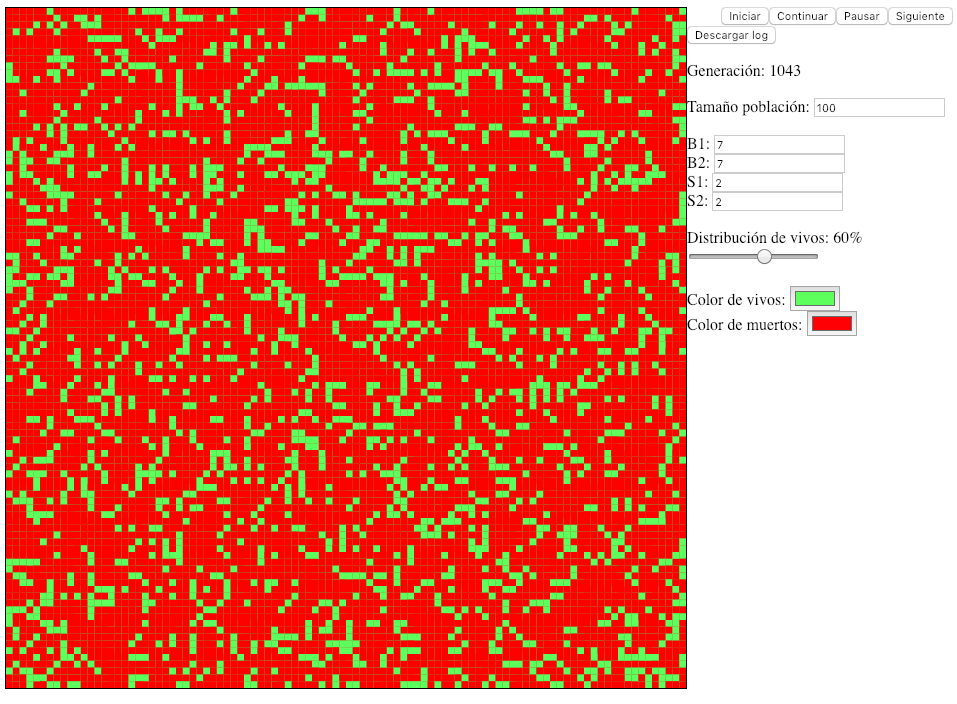
\includegraphics[scale=.3]{GOL/img/dif60-1.png}
			\caption{Regla de difusión con probabilidad de 60\%}
			\label{fig:gol5}
		\end{center}
	\end{figure}

	\begin{figure}[H]
		\begin{center}
			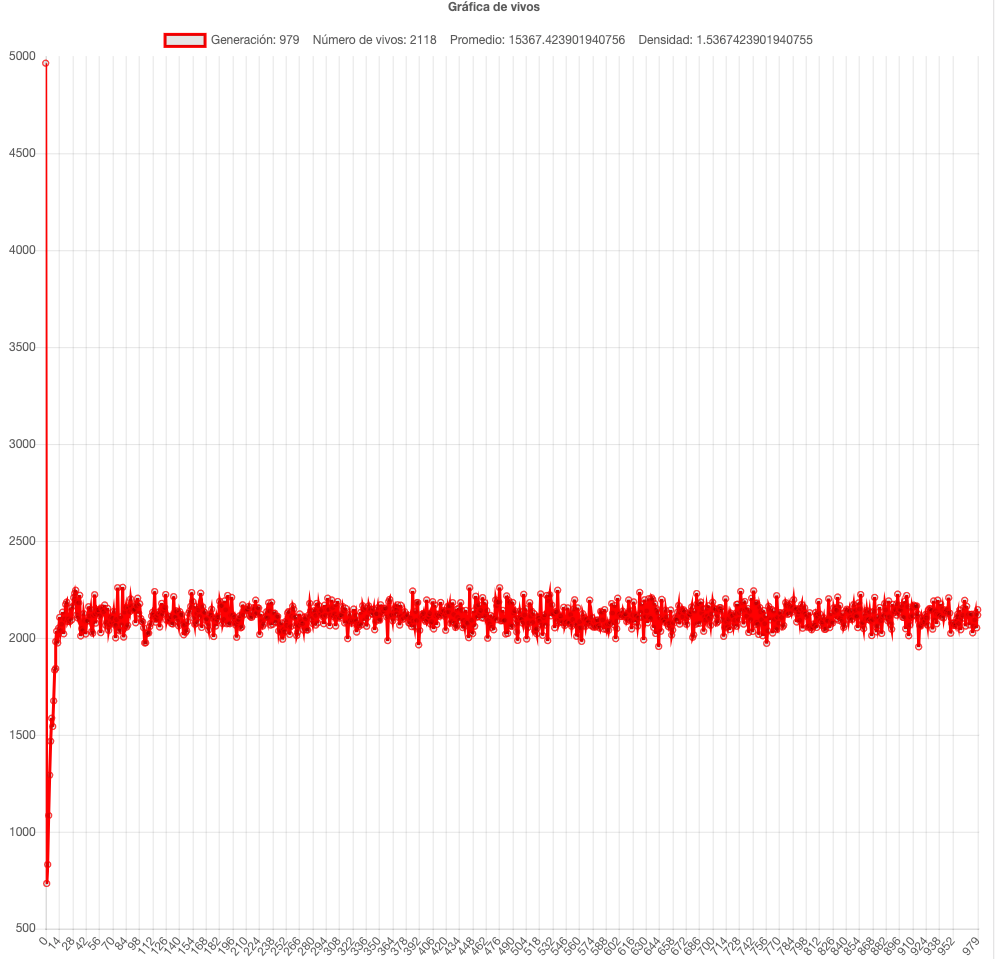
\includegraphics[scale=.24]{GOL/img/dif60-2.png}
			\caption{Comportamiento de la población de la simulación anterior}
			\label{fig:gol5}
		\end{center}
	\end{figure}

	\begin{figure}[H]
		\begin{center}
			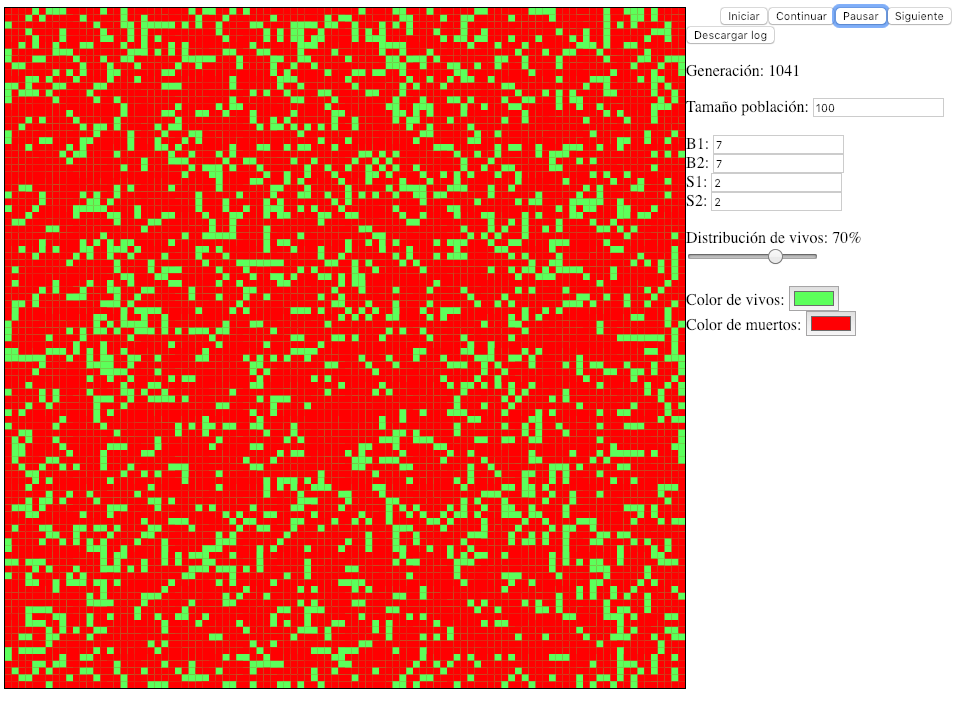
\includegraphics[scale=.3]{GOL/img/dif70-1.png}
			\caption{Regla de difusión con probabilidad de 70\%}
			\label{fig:gol5}
		\end{center}
	\end{figure}

	\begin{figure}[H]
		\begin{center}
			\includegraphics[scale=.24]{GOL/img/dif70-2.png}
			\caption{Comportamiento de la población de la simulación anterior}
			\label{fig:gol5}
		\end{center}
	\end{figure}

	\begin{figure}[H]
		\begin{center}
			\includegraphics[scale=.3]{GOL/img/dif80-1.png}
			\caption{Regla de difusión con probabilidad de 80\%}
			\label{fig:gol5}
		\end{center}
	\end{figure}

	\begin{figure}[H]
		\begin{center}
			\includegraphics[scale=.24]{GOL/img/dif80-2.png}
			\caption{Comportamiento de la población de la simulación anterior}
			\label{fig:gol5}
		\end{center}
	\end{figure}

	\begin{figure}[H]
		\begin{center}
			\includegraphics[scale=.3]{GOL/img/dif90-1.png}
			\caption{Regla de difusión con probabilidad de 90\%}
			\label{fig:gol5}
		\end{center}
	\end{figure}

	\begin{figure}[H]
		\begin{center}
			\includegraphics[scale=.24]{GOL/img/life90-2.png}
			\caption{Comportamiento de la población de la simulación anterior}
			\label{fig:gol5}
		\end{center}
	\end{figure}

Para la regla de difusión se podria decir que el comportamiento de la población es más estable que la de life, debido a que en todas las simulaciones la cantidad de vivos que se graficaban no era tan variable desde un inicio y el comportamiento de la gráfica es igual en todas las probabilidades de uno que se probaron en donde la población oscila entre un limite mayor y uno menor.

% \newpage
% \subsection{Conclusiones}
	El uso de autómatas finitos deterministas y no deterministas nos permite validar que el orden en cadenas de entrada sea correcto.
	Esto tiene diversas aplicaciones, desde muy sencillas (como validar el formato de un CURP) hasta aplicaciones más complejas como realizar parte del análisis léxico de un lenguaje de entrada en un compilador.\\Los cuales nos ayudan a saber si una entrada pertenece a nuestro lenguaje o no, siendo de gran utilidad al momento de validar cadenas apartir de una expresión regular.

\bibliographystyle{ieeetr}
\bibliography{referencias}

%\cite{macy}

\end{document}
